

\chapter{Notational Conventions and Preliminaries}
%\addcontentsline{toc}{chapter}{Notational Conventions and Preliminaries}

\label{ch-conventions}
\section{Some abbreviations frequently
used throughout this book}

\begin{itemize}
\item
AI/ML  = Artificial Intelligence/Machine Learning
\item
bnet= Bnet= Bayesian Network
\item
CPT = Conditional Probabilities Table,
 same as TPM
\item
DAG = Directed Acyclic Graph
\item
i.i.d.= independent identically
distributed.
 \item
 RCT= Randomized Controlled Trial,
a.k.a. A/B testing.

\item
TPM= Transition Probability Matrix,
same as CPT

\end{itemize}

\section{Drawing Bayesian Networks}
Most B nets (also Petri nets, Finite State Machines and Turing Machines)
in this book were drawn using the LaTex package {\tt
 xy-pic} (xypic), or the Python app {\tt texnn} (Ref.\cite{texnn}). {\tt texnn} is a Python wrapper for
{\tt xy-pic} that I wrote specially for this book.

Simple trees in this book were also
drawn using {\tt xy-pic}, but more complicated
ones were drawn using the LaTex packages {\tt istgame}
and {\tt dirtree}.


\section{${\cal N}(!a)$}
$\caln(!a)$ will denote
a normalization constant that does not depend
on $a$. For example, $P(x)=\caln(!x)e^{-x}$
where $\int_0^\infty dx \;P(x)=1$.

\section{Indicator function
(a.k.a. Truth function)}
\beq
\indi(\cals)=\left\{
\begin{array}{l}
1\;{\rm if\; \cals\; is\; true}
\\
0 \;{\rm if \;\cals\; is \;false}
\end{array}
\right.
\eeq
For example, $\delta(x,y)=\indi(x=y)$.


\section{One hot vector}
A {\bf one hot  vector}
is a vector with all entries
equal to zero with
the exception of a single entry which is one.
A {\bf one cold vector}  is a vector with all entries
equal to one with the exception of  a
single entry which is zero.
For example, if $x^n=(x_0, x_1, \ldots,
x_{n-1})$ and
$x_i=\delta(i,0)$ then $x^n$ is one hot.

Two types of
sets that one frequently encounters
are {\bf categorical sets} (a.k.a. \qt{nominal sets}, i.e.,
sets with \qt{named} elements, with elements given a \qt{nomme})
and {\bf numerical sets} (a.k.a. \qt{ordinal sets}, i.e., sets
 with \qt{ordered}
elements).
For example, $\{1,2,5\}$ is a numerical set
because its elements have a natural order,
and $\{\text{cat, dog, bird}\}$ is a  categorical set
because its elements don't have a natural order.

In Machine Learning (ML),
one often encodes categorical sets as one-hot vectors.
For example, suppose we have 4 binary registers (i.e., nodes)
 $x_3, x_2,x_1, x_0$
and  the categorical set $\{\text{cat, dog, canary}\}$.
Then a possible {\bf one-hot encoding}
of the set
is cat=0001, dog=0010 and canary=0100.
This differs from
a {\bf binary encoding} of the set such as
cat=0000, dog=0001, canary=0011.
Clearly, a binary encoding requires
fewer registers than a one-hot
encoding to
encode the same set,
and the one-hot encoding
of a set with $n$ elements requires
$n$ or more registers.

\section{$L^p$  norm}
\label{sec-p-norm}

For $p\in [0, \infty]$
and $\vec{x}\in\RR^n$ or $\vec{x}\in\CC^n$ (note that $n$ and $p$ are generally not the same),
the {\bf $L^p$ norm} $\norm{\vec{x}}_p$ of $\vec{x}$
is defined as

\beq
\norm{\vec{x}}_p
 = \left(\sum_{i=1}^n |x_i|^p
\right)^{\frac{1}{p}}
\eeq
For example,


\beq
\norm{\vec{x}}_0 = \sum_{i=1}^n \indi(|x_i| >0) = \text{number of non-zero $x_i$}
\eeq

\beq
\norm{\vec{x}}_1 = \sum_{i=1}^n |x_i|
\eeq

\beq
\norm{\vec{x}}_2 = \sqrt{\sum_{i=1}^n (x_i)^2}
\eeq

\beq
\norm{\vec{x}}_3 = \left(\sum_{i=1}^n |x_i|^3
\right)^\frac{1}{3}
\eeq

\beqa
\norm{\vec{x}}_\infty
&=&
\lim_{p\rarrow\infty}
\norm{\vec{x}}_p
\\
&=&
\lim_{p\rarrow\infty}((\max_i|x_i|)^p)^{\frac{1}{p}}
\;\; \text{(because one $|x_i|^p$ dominates the rest)}
\\
&=&
\max_i|x_i|
\eeqa

Note that as $\lim_{p\rarrow 0}\norm{\vec{x}}_p \neq  \norm{\vec{x}}_0$. In fact, as $p\rarrow 0$,

\beqa
\norm{\vec{x}}_p&\rarrow&
(\text{number of non-zero $x_i$})^{\frac{1}{p}}\;\;
\text{(because $|x|^0=1$ for $x\neq  0$)}
\\
&\rarrow&
\norm{\vec{x}}_0^{\frac{1}{p}}
\rarrow \infty
\eeqa

When $n$ is large and only a few
of the $n$ components of $\vec{x}\in\CC^n$ are non-zero, we say
$\vec{x}$ is {\bf sparse}. $\norm{\vec{x}}_0$ is used to measure
the {\bf sparsity} of vectors.

Fig.\ref{fig-normballs.png} shows the {\bf unit balls}
$\{\vec{x}\in \RR^n:\norm{\vec{x}}_p\leq 1\}$ for various values of $p$ and for $n=2$.
$\{\vec{x}\in \RR^2:\norm{\vec{x}}_0\leq 1\}$ is not shown. It equals all the $x$ and $y$ axes, because, by definition, it contains all $(x,y)\in\RR^2$ such that $x=0$ or $y=0$ or both (i.e., 0 or 1 non-zero components).

\begin{figure}[h!]
\centering
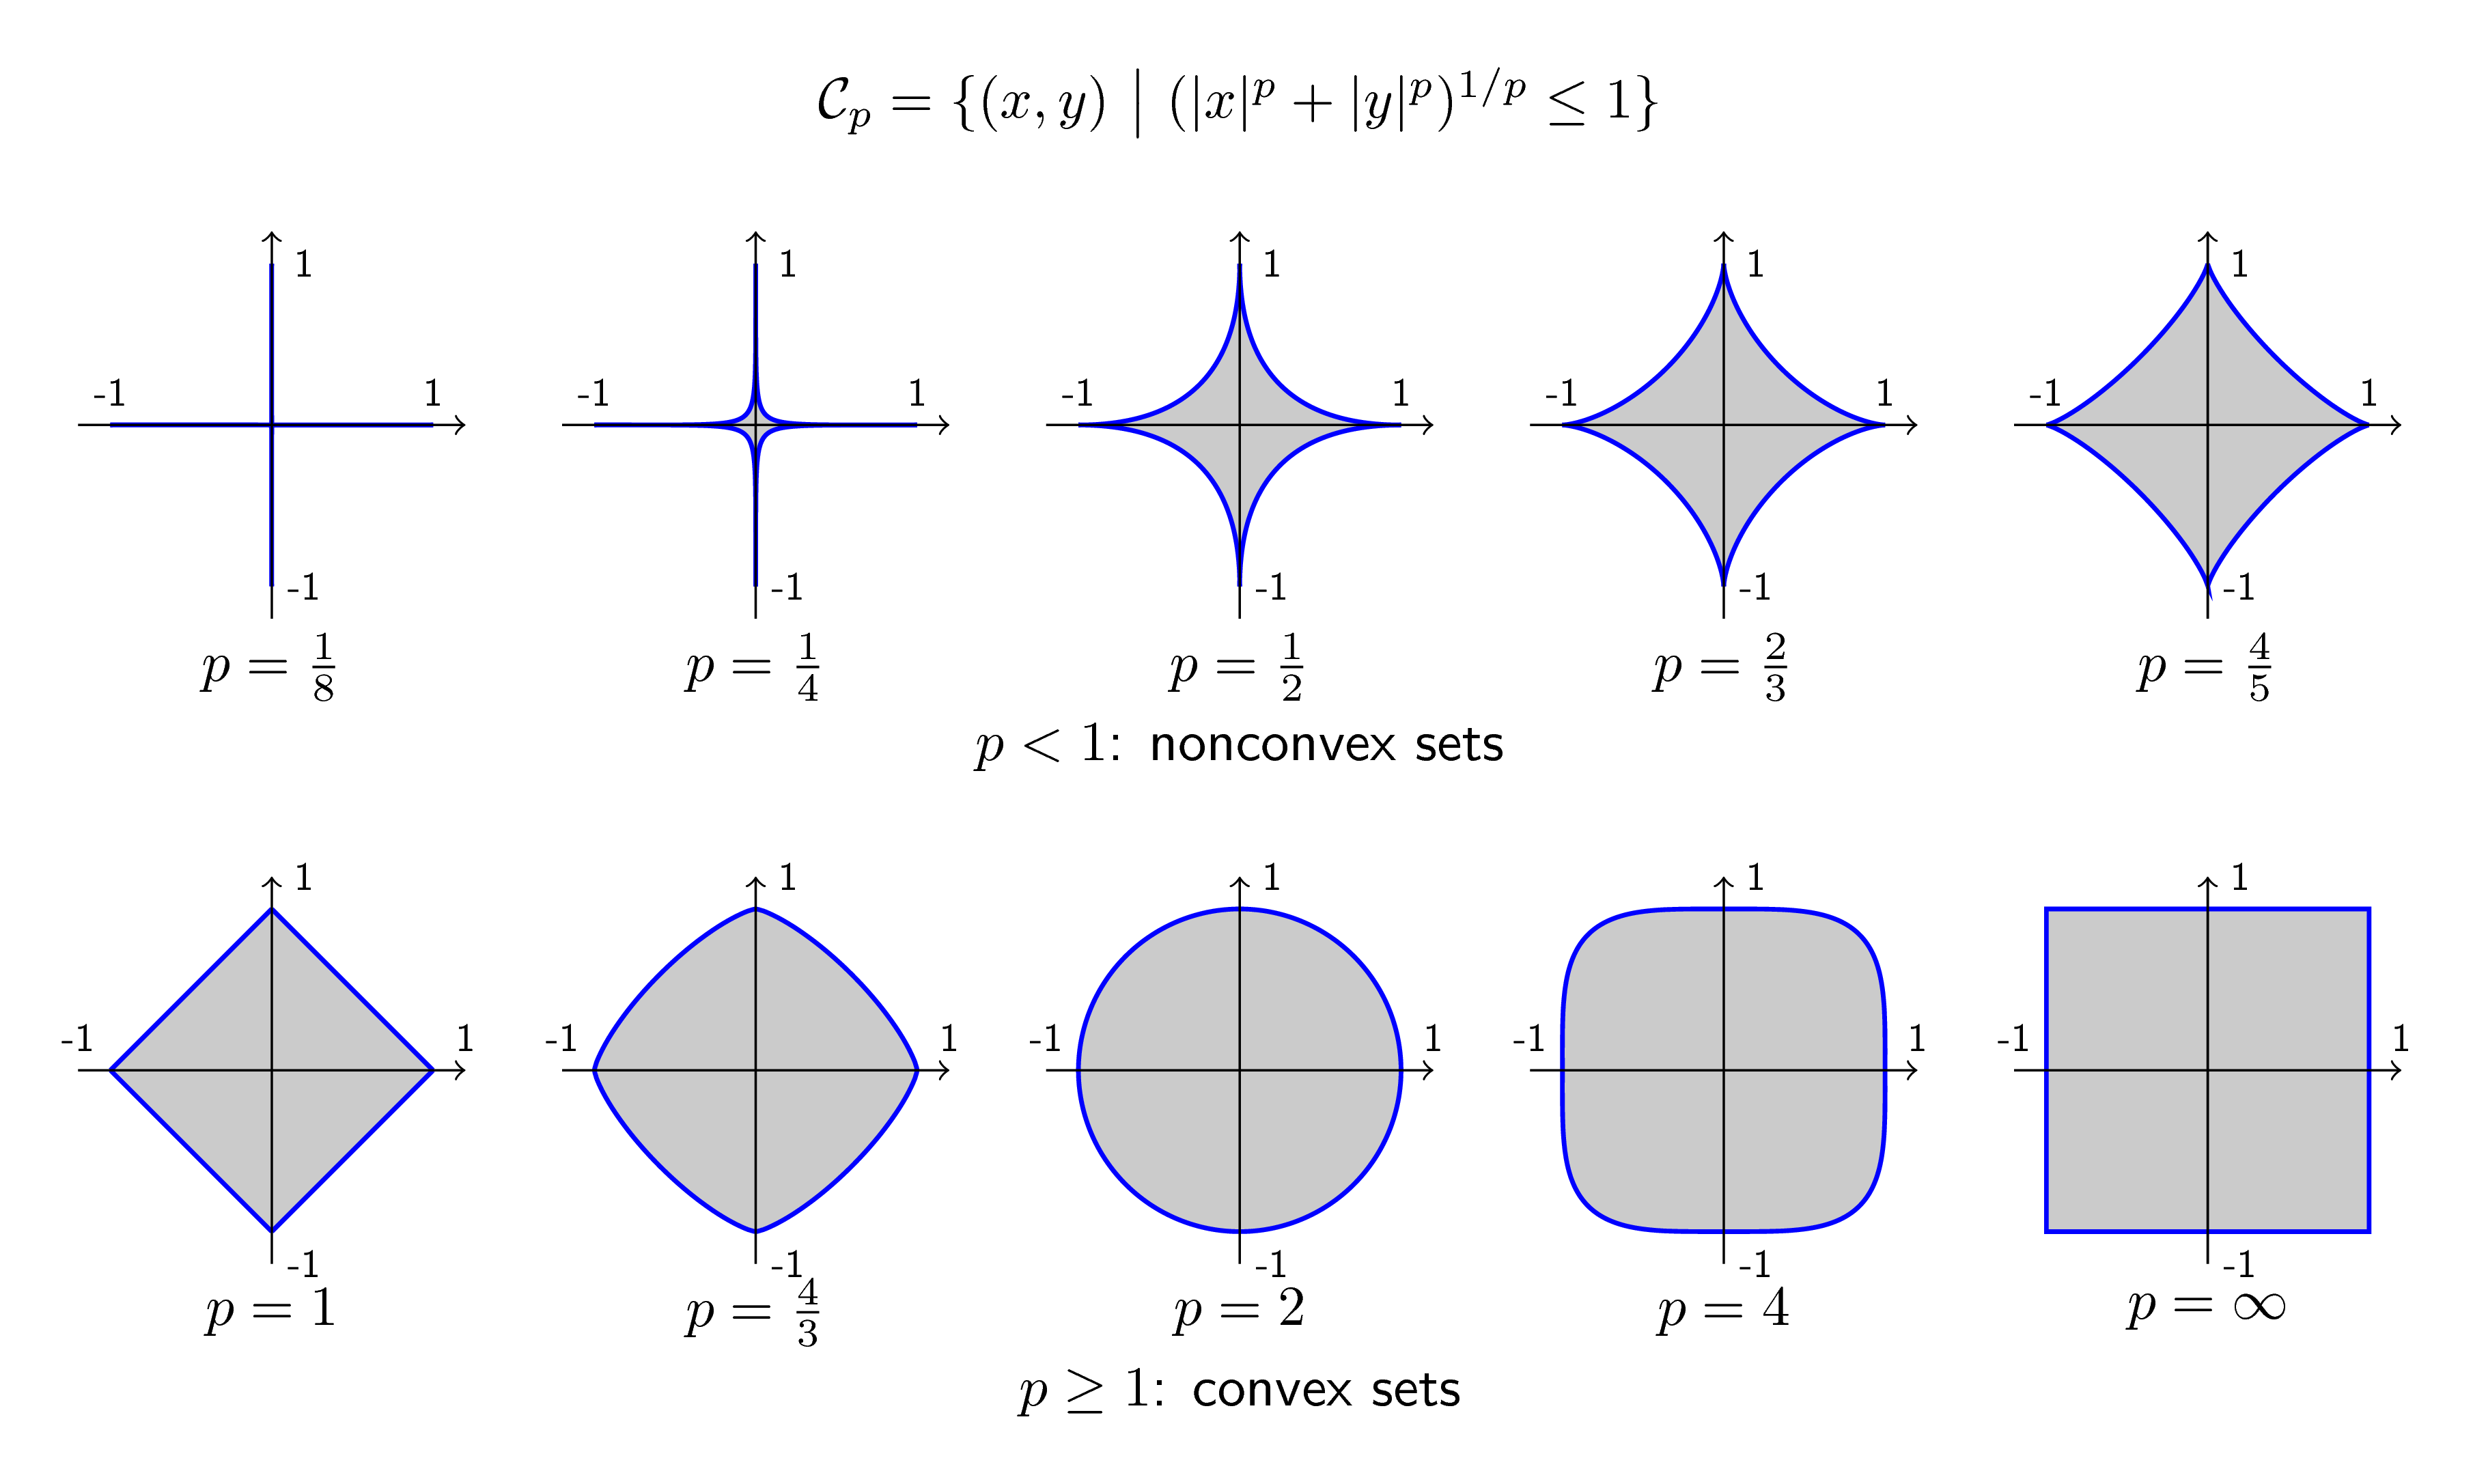
\includegraphics[width=6in]
{conventions/normballs.png}
\caption{Unit Balls
$\{\vec{x}\in \RR^n:\norm{\vec{x}}_p\leq 1\}$  for various values of $p$ and for $n=2$.
}
\label{fig-normballs.png}
\end{figure}



\section{Special sets}
Define $\ZZ, \RR, \CC$ to be
 the integers, real numbers
 and complex numbers, respectively.

For $a<b$, define $\ZZ_I$
to be the integers in the
interval $I$, where
$I=[a,b],[a,b),(a,b],(a,b)$
(i.e, $I$ can be closed or
 open on either side).

$A_{>0}=\{k\in A: k>0\}$ for $A=\ZZ, \RR$.

\section{Kronecker
delta function}

 For $x,y$ in discrete set $S$,
\beq
\delta(x,y)=\left\{
\begin{array}{l}
1\;{\rm if}\; x=y
\\
0 \;{\rm if}\; x\neq y
\end{array}
\right.
\eeq

\section{Dirac delta function}
 For $x,y\in\RR$,
\beq
\int^{+\infty}_{-\infty}dx\;\delta(x-y)f(x)=f(y)
\eeq


\section{Majority function}
The {\bf majority function}  is defined as follows.

\beq
\begin{array}{ll}
{\tt majority}(L)=&
\text{ most common element of  list $L$}
\\
&\text{(ties resolved by chance)}
\end{array}
\eeq
Note that the majority function
acts on lists, not sets. By definition,
all elements of a set appear only once in the set.
${\tt majority}(L)$
is usually
used when the elements of
$L$ are categorical (i.e., not real numbers).
When they are real numbers,
it makes more sense to use, instead of
${\tt majority}(L)$, a simple average
of the elements of $L$.


\section{Underlined letters
 indicate random variables}
Random variables will be indicated by
underlined letters and their values
by non-underlined letters.
 Each node of a bnet will be
 labeled by a random variable.
 Thus, $\rvx=x$ means that node
$\rvx$ is in state $x$.

It is more
conventional to
use an upper
case letter to
indicate
a random
variable
and a lower case letter
for its state.
Thus, $X=x$ means that
random variable
$X$ is in state $x$.
However,
we have
opted
in this
book to
avoid
that notation,
because
we often
want to define
certain lower
case letters
to be random variables
or, conversely, define certain upper
case letters to
be non-random variables.

\section{Probability distributions}
 $P_\rvx(x)=P(\rvx=x)=P(x)$ is the probability that random variable $\rvx$ equals $x\in val(\rvx)$. $val(\rvx)$ is the set of states (i.e., values) that $\rvx$ can assume and $n_\rvx = |val(\rvx)|$ is the size (a.k.a. cardinality) of that set. Hence,
\beq
\sum_{x\in val(\rvx)}P_\rvx(x)=1
\eeq

\hrule
\beq
P_{\rvx,\rvy}(x,y)=P(\rvx=x, \rvy=y)=P(x,y)
\eeq
\beq
P_{\rvx|\rvy}(x|y)=P(\rvx=x| \rvy=y)=P(x|y)=\frac{P(x,y)}{P(y)}
\eeq

\section{Independence, $\perp_P$}
\label{sec-perp-p}

Two variables $\rva$ and $\rvb$
are said to be {\bf independent} if

\beq
P(a,b)=P(a)P(b)
\eeq
or,
equivalently, when $P(b)\neq 0$,

\beq
P(a|b)=P(a)
\eeq
In such a case, we write $\rva\perp_P \rvb$
or just $\rva\perp \rvb$ if
the distribution $P$
being alluded to is clear.
Note that
$\rva\perp \rvb$ iff
$\rvb\perp \rva$.


Two variables $\rva$ and $\rvb$ are
said to be {\bf conditionally independent at fixed $\rvz$} if

\beq
P(a,b|z)=P(a|z)P(b|z)\eeq
or, equivalently, if $P(b|z)\neq 0$,

\beq
P(a|b,z)=P(a|z)
\eeq
In such a case, we write $\rva\perp_P \rvb|\rvz$
or just $\rva\perp \rvb|\rvz$ if
the distribution $P$
being alluded to is clear.
Note that
$\rva\perp \rvb|\rvz$ iff
$\rvb\perp \rva|\rvz$.


In
this book, we use both
$(\rva, \rvb)\perp^{sep} \rvx$
and $(\rva, \rvb)\perp^{joint} \rvx$.

When we write $(\rva, \rvb)\perp^{sep} \rvx$,
we mean that
$\rva\perp \rvx$
and $\rvb\perp\rvx$ separately; that is,
$P(a|x)=P(a)$
and $P(b|x)=P(b)$.

When we write
$(\rva, \rvb)\perp^{joint} \rvx$
or simply $(\rva, \rvb)\perp \rvx$,
we mean $P(a,b|x)=P(a,b)$.

\begin{claim}
$(\rva, \rvb)\perp^{joint} \rvx$
implies
$(\rva, \rvb)\perp^{sep} \rvx$
\end{claim}
\proof
Summing
$P(a,b|x)=P(a,b)$
over $a$ gives
$P(b|x)=P(b)$,
and summing it
over $b$ gives
$P(a|x)=P(a)$.\qed

\begin{claim}
Assume
$(\rva,\rvb)\perp^{sep} \rvx$
and $\rva\perp\rvb$. Then
$(\rva, \rvb)\perp^{joint} \rvx$
iff
$(\rva, \rvb)\perp^{sep} \rvx$.
\end{claim}
\proof
We already know that $(\rva, \rvb)\perp^{joint}\rvx$ implies $(\rva, \rvb)\perp^{sep}\rvx$.
To prove the converse, note that
$(\rva, \rvb)\perp^{sep}\rvx$ means

\beq
P(a|x)=P(a)\;,\;\; P(b|x)=P(b)
\eeq
Hence

\beq
P(a,b|x)=P(a|x)P(b|x)=P(a)P(b)=P(a,b)
\eeq
\qed

\section{Discretization
of continuous
probability distributions}

The TPM of a node
of a bnet can be either a discrete or
a continuous probability distribution.
To go from continuous to discrete, one
replaces integrals over states of a node
 by sums over new states, and Dirac delta
functions by Kronecker delta functions.
 More precisely, consider a function
$f: [a, b]\rarrow \RR$. Express
 $[a,b]$ as
a union of
small, disjoint (except for
one point) closed sub-intervals (bins) of
length $\Delta x$.
Name one point
in each bin to be the representative of that bin,
and  let $val(\rvx)$ be the
set of all the bin representatives. This is called
discretization or binning. Then

\beq
\frac{1}{(b-a)}
\int_{[a,b]} dx \; f(x)\rarrow
\frac{\Delta x}{(b-a)} \sum_{x\in val(\rvx)}f(x)
=
\frac{1}{n_\rvx} \sum_{x\in val(\rvx)}f(x)
 \;.
\eeq
Both sides of last equation are 1 when $f(x)=1$.
 Furthermore, if $y\in val(\rvx)$, then

\beq
\int_{[a,b]} dx \; \delta(x-y)f(x)=f(y)
\rarrow \sum_{x\in val(\rvx)}\delta(x,y)f(x)
=f(y)
\;.
\eeq

As usual in this book, let $val(\rvx)$ denote the set of
values that the random variable $\rvx$ can take.
When $val(\rvx)\subset \RR$,
we will assume that $val(\rvx)$
for a probability distribution $P(x)$
can be either a discrete or a continuous
subset of $\RR$.\footnote{By a \qt{continuous set} we
mean a finite set of intervals
 each of which has non-zero length.}
When $val(\rvx)$ is a discrete subset of $\RR$, $P(x)$
will denote a probability distribution
for which $\sum_{x\in val(\rvx)}P(x)=1$, whereas when
$val(\rvx)$ is continuous, $P(x)$ will denote
a probability density
for which $\int_{x\in val(\rvx)}dx\; P(x)=1$.

\section{Samples,
i.i.d. variables}
\beq
\vec{x}= (x[0], x[1], x[2] \ldots,
 x[nsam(\vecx)-1])=x[:]
\eeq

 $nsam(\vecx)$ is the number of samples
 of $\vecx$.
$\rvx[\sigma]\in val(\rvx)$ are
 i.i.d. (independent identically distributed)
samples with

 \beq
x[\sigma]\sim P_\rvx\;\;({\rm i.e.}\; P_{\ul{x[\sigma]}}=P_\rvx)
\eeq

\beq
P(\rvx=x)=\frac{1}{nsam(\vecx)}\sum_\sigma \indi(x[\sigma]=x)
\eeq
Hence, for any $f:val(\rvx)\rarrow \RR$,
\beq
\sum_x P(\rvx=x)f(x)
=\frac{1}{nsam(\vecx)}\sum_\sigma f(x[\sigma])
\eeq


If we use two sampled variables, say $\vecx$ and $\vecy$,
in a given bnet, their number of samples
$nsam(\vecx)$ and $nsam(\vecy)$ need not be equal.

\hrule
\beq
P(\vecx) = \prod_\sigma P(x[\sigma])
\eeq

\beq
\sum_\vecx = \prod_\sigma\sum_{x[\sigma]}
\eeq

\beq
\partial_\vecx =
[\partial_{x[0]}, \partial_{x[1]},\partial_{x[2]}, \dots, \partial_{x[nsam(\vecx)-1]}]
\eeq

\hrule
\beqa
P(\vecx)&\approx& [\prod_x P(x)^{P(x)}]^{nsam(\vecx)} \\
&=& e^{nsam(\vecx)\sum_x P(x)\ln P(x)}\\
&=& e^{-nsam(\vecx)H(P_\rvx)}
\eeqa

\section{Expected Value and Variance}

Given a random variable
 $\rvx$ with states $val(\rvx)$ and
a function $f:val(\rvx)\rarrow \RR$, define

\beq
E_\rvx[f(\rvx)]=
E_{x\sim P(x)}[f(x)] = \sum_x P(x) f(x)
\eeq

\beqa
Var_\rvx[f(\rvx)]&=& E_\rvx
\left[(f(\rvx)-E_\rvx[f(\rvx)])^2\right]
\\
&=&
E_\rvx[f(\rvx)^2]-(E_\rvx[f(\rvx)])^2
\eeqa

\beq
E[\rvx]=E_\rvx[\rvx]
\eeq

\beq
Var[\rvx]=
Var_\rvx[\rvx]
\eeq



\section{Conditional Expected Value}

Given a random variable $\rvx$ with states $val(\rvx)$, a random variable $\rvy$ with states $val(\rvy),$ and a function $f:val(\rvx)\times val(\rvy)\rarrow \RR$, define

\beq
E_{\rvx|\rvy}[f(\rvx, \rvy)]=
\sum_x P(x|\rvy) f(x, \rvy)
\;,
\eeq

\beq
E_{\rvx|\rvy=y}[f(\rvx, y)]=
E_{\rvx|y}[f(\rvx, y)]= \sum_x P(x| y) f(x, y)
\;.
\eeq
Note that

\beqa
E_\rvy[E_{\rvx|\rvy}[f(\rvx, \rvy)]]&=&
\sum_{x,y}P(x|y)P(y)f(x,y)
\\&=&
\sum_{x,y}P(x,y)f(x,y)
\\&=&
E_{\rvx, \rvy}[f(\rvx, \rvy)]
\;.
\eeqa



\section{Notation
for covariances}
\label{sec-notation-cov}

Consider two random variables $\rvx, \rvy$.

\begin{itemize}
\item
Mean value of $\rvx$
\beq
\av{\rvx}=
E_\rvx[\rvx]
\eeq

\item
Signed distance of $\rvx$ to its mean value
\beq
\Delta \rvx = \rvx - \av{\rvx}
\eeq

\item
Covariance of $(\rvx, \rvy)$
\beq
Cov(\rvx, \rvy)=\av{\rvx, \rvy}=
\av{\Delta \rvx \Delta \rvy}
=
\av{\rvx\rvy}-\av{\rvx}\av{\rvy}
\eeq

$\av{\rvx, \rvy}$ is symmetric
(i.e., $\av{\rvx, \rvy}=\av{\rvy, \rvx}$)
and bilinear (i.e.,
$\av{\sum_i \alp_i\rvx_i, \rvy}
=
\sum_i\alp_i\av{\rvx_i, \rvy}$, where
$\alp_i\in \RR$
are non-random scalars
and $\rvx_i, \rvy\in\RR$ are
real-valued random
variables.)

\item
Variance of $\rvx$
\beq
Var(\rvx)=\av{\rvx, \rvx}
\eeq

\item
Standard deviation or $\rvx$
\beq
\sigma_\rvx=\sqrt{\av{\rvx, \rvx}}
\eeq

\item
Correlation Coefficient of $(\rvx, \rvy)$
\beq
\rho_{\rvx, \rvy}=
\frac{\av{\rvx, \rvy}}
{\sqrt{\av{\rvx, \rvx}\av{\rvy, \rvy}}}
\eeq

\item Partial derivative of $\rvy$
wrt (i.e., with respect to) $\rvx$

\beq
\partial_\rvx\rvy
=
\pder{\rvy}{\rvx}
=
\frac{\av{\rvx,\rvy}}
{\av{\rvx, \rvx}}
=
\rho_{\rvx, \rvy}\frac{
\s_\rvy}
{\s_\rvx}
\eeq
\end{itemize}


\section{Conditional Covariance}
\label{sec-cond-cov}
Let $\rvx, \rvy, \rva$
be random variables.
The covariance $Cov(\rvx, \rvy|\rva=a)$
of $\rvx$ and $\rvy$
given $\rva=a$, is defined
the same
way as $Cov(\rvx, \rvy)$,
except that all
expected values are
conditioned on $\rva=a$.



\beq
Cov(\rvx, \rvy|\rva=a)=
\av{\rvx, \rvy}^{|a}
=
\av{(\rvx-\av{\rvx}^{|a})
(\rvy-\av{\rvy}^{|a})}^{|a}
\eeq
where

\beq
\av{\rvx}^{|a}=E_{\rvx|a}[\rvx]
\;.
\eeq

In this book, we will use the following notation
for conditional averages.
For any random
variables $\rvx, \rvy, \rva$, let

\beq
E_{|a}[\rvx]=\av{\rvx}^{|a}
\quad\text{(mean)}
\eeq

\beq
\av{\rvx, \rvy}^{|a}=
\av{\rvx\rvy}^{|a}
-
\av{\rvx}^{|a}\av{\rvy}^{|a}
\quad\text{(covariance)}
\eeq

\beq
\s_\rvx^{|a} =\sqrt{\av{\rvx, \rvx}^{|a}}
\quad \text{(standard deviation)}
\eeq

\beq
\rho_{\rvx, \rvy}^{|a}
=
\frac{\av{\rvx, \rvy}^{|a}}
{\s_\rvx^{|a} \s_\rvy^{|a}}
=
\left[
\frac{\av{\rvx, \rvy}}
{\s_\rvx \s_\rvy}
\right]^{|a}
\quad \text{(correlation)}
\eeq

\beq
\partial_\rvx^{|a}\rvy
=
\left[\pder{}{\rvx}\right]^{|a}\rvy
=
\frac{\av{\rvx,\rvy}^{|a}}
{\av{\rvx, \rvx}^{|a}}
=
\rho_{\rvx, \rvy}^{|a}\frac{
\s_\rvy^{|a}}
{\s_\rvx^{|a}}
=
\left[
\rho_{\rvx, \rvy}\frac{
\s_\rvy}
{\s_\rvx}\right]^{|a}
\quad\text{(partial derivative)}
\eeq
\qt{$|a$} means that the variable
$\rva$ is held fixed to $a$
when taking all averages.





\section{Normal Distribution}


For $x, \mu, \sigma\in \RR$,
$\sigma >0$, we define the Normal Distribution
(see Fig.\ref{fig-norm-dist}) by

\beq
\caln(x; \mu, \sigma^2)=
\frac{1}{\sigma\sqrt{2\pi}}
e^{-\;\frac{1}{2}\left(
\frac{x-\mu}{\sigma}\right)^2}
\;.
\eeq

For a {\bf standard deviation}
$\s$, the {\bf precision} $\tau$
is defined as $\tau=\frac{1}{\s^2}$.

\begin{claim}
If

\beq
\rvx_1\sim \caln(\mu_1, \s^2_1)
\eeq
and

\beq
\rvx_2\sim \caln( \mu_2, \s^2_2)
\eeq
then
\beq
\rvx=\rvx_1 +\rvx_2 \sim \caln(\mu_1 + \mu_2, \s^2_1 + \s^2_2)
\;.
\eeq
\end{claim}
\proof

\beqa
P(\rvx=x)&=&\caln(!x)
\int_{-\infty}^{+\infty}dx_2\;
P(\rvx_1 + \rvx_2 = x|\rvx_2=x_2)P(x_2)
\\
&=&\caln(!x)
\int_{-\infty}^{+\infty}dx_2\;
\caln(x-x_2;\mu_1, \s^2_1)
\caln(x_2;\mu_2, \s^2_2)
\\
&=&
\caln(x;\mu_1 +\mu_2; \s^2_1+\s^2_2)
\eeqa
\qed

\begin{figure}[h!]
\centering
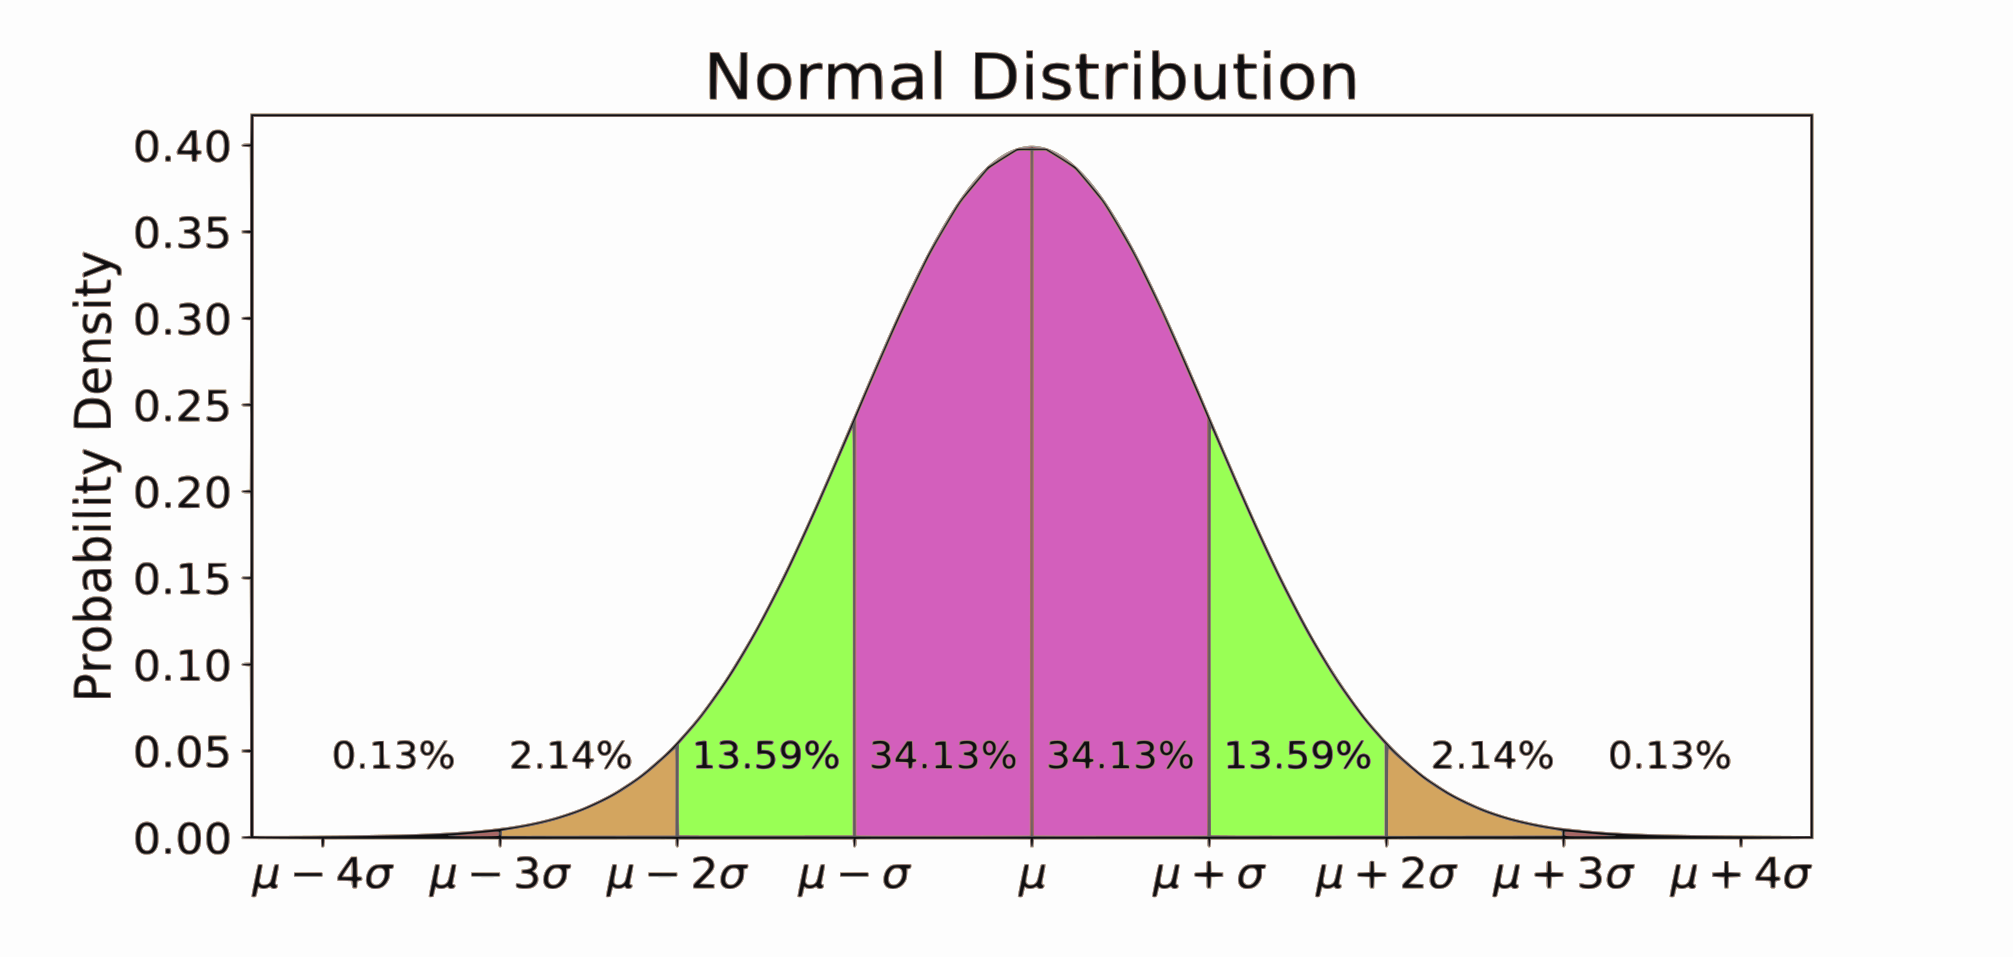
\includegraphics[width=5in]
{conventions/normal-dist.png}
\caption{Normal Distribution
$\caln(x;\mu, \s^2)$.}
\label{fig-norm-dist}
\end{figure}

The {\bf Standard Normal Distribution} $P_{SND}(x)$
and its cumulative distribution $\Phi(x)$ are defined by

\beq
P_{SND}(x)=\caln(x; \mu=0, \s=1)
\eeq

\beq
\Phi(x) = \int_{-\infty}^x dx'\;P_{SND}(x')
\eeq

The {\bf error function} ${\rm erf}:\RR\rarrow [-1,1]$
is defined by
\beq
{\rm erf}(x) = \frac{2}{\sqrt{\pi}}
\int_0^x du \; e^{-\;\frac{u^2}{2}}
\eeq

Note that

\beq
\Phi(x)= \frac{1}{2} + \frac{1}{2}{\rm erf}(x)
\label{eq-Phi-erf}
\eeq
Eq.(\ref{eq-Phi-erf})
is interpreted geometrically in Fig.\ref{fig-erf}.

\begin{figure}[h!]
\centering
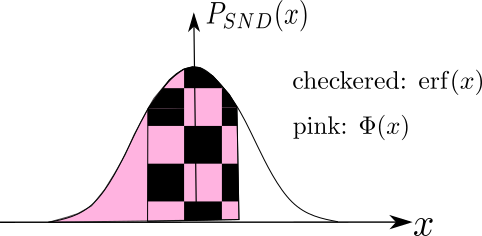
\includegraphics[width=2.8in]
{conventions/erf.png}
\caption{Plot of Standard
Normal Distribution $P_{SND}(x)$.
 Values of ${\rm erf}(x)$ and $\Phi(x)$
 equal indicated areas.}
 \label{fig-erf}
\end{figure}
\section{Uniform Distribution}
For $a<b$, $x\in [a,b]$

\beq
\calu(x;a,b) =
\frac{1}{b-a}
\eeq

\section {Softmax function
(a.k.a. Boltzmann Distribution)}

The Softmax function
 is defined by
\beq
P(x_i
|x.)=\frac{e^{x_i}}{\sum_i e^{x_i}}=
\softmax(x.)(i)
\label{eq-softmax}
\eeq
The
Boltzmann distribution is defined as

\beq
P(\rvE_a=E_a)=\frac{\exp(-\;\frac{E_a}{kT})}{\sum_{a}
\exp(-\;\frac{E_{a}}{kT})}=
P(\frac{-E_a}{kT}|E.)\eeq
for a system with energies $E_a$
and temperature $T$,
where $k$
is Boltzmann's constant.

The function
softmax() is called softmax because if we
approximate the exponentials,
 both in the numerator and denominator
of Eq.(\ref{eq-softmax}),
by the largest one
of them or zero,
we get

\beq
\softmax(x.)(i)\approx \delta(i, \argmax_k x_k)
\;.
\eeq
Thus, $\softmax(x.)(i)$
returns a continuous
function that approximates a
Kronecker delta function.
The softmax function doesn't really
return the soft maximum of a finite set, so
its name is a bit of a misnomer.
A better name for it would have been \qt{soft Kronecker
delta function}.

Note that
\beq
\pder{\ln P(x_i|x)}{x_a}
=
\pder{}{x_a}\ln\left[
\frac{e^{x_i}}{\sum_i e^{x_i}}
\right]
=
\delta(a,i)
-
P(x_a|x)
\eeq

For 2 variables $x_0, x_1$,
\beqa
P(x_0|x.)&=&
\frac{e^{x_0}}{e^{x_0} + e^{x_1}}\\
&=&\smoid(x_0-x_1)
\;,
\eeqa

\beq
P(x_1|x.)=\smoid(x_1-x_0)
\;.
\eeq

\section{Sigmoid and log-odds functions}
\label{sec-smoid}
The {\bf sigmoid (a.k.a. exp-it,  logistic) function} smoid:$\RR\rarrow [0,1]$
is defined by
\beq
\smoid(x)=
\frac{1}{1+e^{-x}}
\eeq
$\smoid()$ is monotonically
increasing with $\smoid(-\infty)=0$,
$\smoid(0)=1/2$
and $\smoid(+\infty)=1$.
Note that for $x<<0$, $\smoid(x)\approx e^x$, which
is why \qt{smoid} is also called \qt{expit}.

\beqa
\smoid(x)+\smoid(-x)&=&
\frac{1}{1+e^{-x}}+\frac{1}{1+e^x}\\
&=&\frac{2+e^x+e^{-x}}{2+e^x+e^{-x}}
\\&=&1
\eeqa


The {\bf log-odds (a.k.a. log-it) function}
lodds:$[0,1]\rarrow \RR$ is defined by

\beq
{\rm lodds}(p)=\ln\frac{p}{1-p}
\eeq
Note that for $0< p<<1$, $\lodds(x)\approx \ln p$,
which is why \qt{lodds} is also called \qt{logit}.

Note that for $x<<1$, $\smoid(x)\approx e^x<<1$,
so $\lodds(e^x)\approx \ln(e^x)=x$.
More generally, it
is easy to check that for any $p\in[0,1]$ and $x\in \RR$,
\beq
\lodds[\smoid(x)]=x
\eeq

\beq
\smoid [\lodds(p)] =p
\eeq
Hence,
$\lodds()$ is the inverse of $\smoid()$ and vice-versa.

\begin{claim}
\beq
\smoid'(x)=\smoid(x)[1-\smoid(x)]
\eeq

\beq
\smoid''(x)=\smoid'(x)[1-2\smoid(x)]
\eeq
\end{claim}
\proof

In this proof, we will
abbreviate $\smoid(x)$ by $s(x)$.
\beq
1-s(x)=1 -\;\frac{1}{1+e^{-x}}=
\frac{e^{-x}}{1+e^{-x}}
\eeq

\beq
s'(x)= \frac{e^{-x}}{(1+e^{-x})^2}
=s(x)[1-s(x)]
\eeq

\beqa
s''(x)&=&s'(x)[1-s(x)]
+
s(x)(-1)s'(x)
\\
&=&
s'(x)[1-2s(x)]
\\
&=&
s(x)[1-s(x)][1-2s(x)]
\eeqa
\qed

\section{Estimand, Estimator (curve-fit), Estimate, Bias}
\label{sec-estimand}
For an {\bf estimand} $\theta$,
an {\bf estimator (a.k.a. curve-fit)} $\ul{\HAT{\theta}}$
gives {\bf estimate} $E[\ul{\HAT{\theta}}(\theta)]=\theta+b$
with {\bf bias} $b$.
We say this estimate is an {\bf unbiased estimate}
if $b=0$.

Note that, strictly
speaking, an estimator is a function
waiting to be averaged over
and denoted by a letter with a hat,
whereas an estimate is a real number
denoted by a letter without a hat.
Unfortunately, the
words \qt{estimator} and
\qt{estimate} are often used interchangeably,
as if they were synonyms.
And often the estimate $\theta + b$
is denoted by a letter with a hat too.
In some sense, an estimator is an estimate
of a curve, so it's understandable that
the terms \qt{estimator} and \qt{estimate}
are used synonymously.
In this book, we will bow to traditional
practice and
also use
the terms \qt{estimator} and \qt{estimate}
synonymously, and use a letter
with a hat to denote either of them.
This is not
ambiguous as long as we don't
use the same letter with a
hat to denote two different quantities, of course.
When we need to distinguish semantically
between the real value and the function,
we will call the function a curve-fit,
and the real value the estimate.

\section{Maximum Likelihood Estimate,
Likelihood Ratio Test}
\label{sec-likelihood-ratio}

Given a bnet, let $P(x|\theta)$
be its full joint probability distribution,
where
$x$ denotes the joint state
of all the nodes and $\theta$
denotes all the parameters.
 $P(x|\theta)$ is often
called the {\bf likelihood function of $\theta$}
and is denoted by

\beq
L(\theta)= P(x|\theta)
\eeq
It's called a likehood of $\theta$
because, even though it's a probability,
it isn't the probability of $\theta$,
but rather of $x$.

The value of $\theta$
that we obtain by maximizing $L(\theta)$
over $\theta$ is called
the
{\bf maximum likelihood
estimate (MLE) of $\theta$}. Let us denote it by
$\HAT{\theta}$. Note that\footnote{\qt{sup} stands for supremum.
It's a generalization of the function $\max()$
to arbitrary sets
that might not be discrete or finite.
If $S$ is a
finite set,
then $\sup_{\theta\in S} f(\theta)=
\max_{\theta\in S} f(\theta)$
for any function $f:S\rarrow \RR$.
Likewise, \qt{inf} stands for infimum,
and it generalizes the $\min()$ function.}

\beq
\sup_{\theta\in S}L(\theta)=
L(\HAT{\theta})
\eeq


Let $S_0, S_1$ be disjoint sets such that
 $S=S_0\cup S_1$.
We'll say
the {\bf null hypothesis $H_0$} holds
 if $\theta\in S_0$,
and the {\bf alternative hypothesis $H_1$}
holds if
$\theta\in S_1$.
The {\bf likelihood ratio (LR) test statistic}
is defined by


\beq
R=-2\ln
\left(\frac{\sup_{\theta\in S_0}L(\theta)}
{\sup_{\theta\in S}L(\theta)}\right)
\eeq
$R\geq 0$ and $R=0$ if  $S_0=S$.
For some small $c>0$,
if $R<c$, then we reject the alternative hypothesis,
and if $R>c$, we accept it.




If $S_0=\{\theta_0\}$,
then

\beq
R= -2[\ln L(\theta_0) -\ln L(\HAT{\theta})]
\eeq


\section{Mean Square Error (MSE)}

Suppose we are
given $nsam$ samples $y^\s\in\RR$
labeled by an index $\s$,
and a curve-fit $\haty^\s(a)\in\RR$
that depends on a parameter $a\in\RR$.
Define the {\bf Mean Square
Error (MSE)}
by

\beq
MSE(a) = \frac{1}{nsam}\sum_\s (y^\s-\haty^\s(a))^2
\;.
\eeq
For example, in Linear Regression (LR),
we have $\haty^\s= a_0 + a_1 x^\s$
where $a=(a_0, a_1)$ is a deterministic
parameter.
If the samples $y^\s$
are i.i.d,
then we can also write


\beq
MSE(a)=E_{|a}[(\rvy-\ul{\haty}(a))^2]
\;.
\eeq
and for LR, $\ul{\haty}(a)=a_0+a_1\rvx$.

Define the {\bf residual} $\Delta\rvy$ by:


\beq
\Delta\rvy(a) =\rvy-\ul{\haty}(a)
\;\;\;\text{ (Hence
$\rvy=\ul{\haty} + \Delta\rvy$)}
\eeq

In the rest of this section,
we will discuss the case that
$\haty^\s(a)$ is independent of $x^\s$.
I call
this the {\bf deterministic MSE (D-MSE)}
model.
Note that this
is different from the LR
case where
$\haty^\s(a)$ does depend on $x^\s$.
In LR, we are trying
to fit
a line to a cigar-shaped
2-D scatter plot.
Here, we are just trying
to estimate
the mean value (center of mass)
of a scatter plot.


\begin{claim}
MSE is minimized
over all functions $\haty$ if
\beq
\haty =E_{|a}[\rvy]
\eeq
\end{claim}
\proof

\beq
MSE = E_{|a}[\rvy^2]-2\haty E_{|a}[\rvy]+ \haty^2
\eeq

\beq
0=\frac{d}{d\haty} MSE = 2(-E_{|a}[\rvy]+\haty)
\eeq
Hence,
\beq
\haty =E_{|a}[\rvy]
\eeq
\qed

Sometimes, we will
use the notation
\beq
\haty_{MSE} = E_{|a=a_{MSE}}[\rvy]
\;.
\eeq

\begin{claim}
Suppose $f(a)$
is a function of $a$.
If $\haty=E_{|a}[\rvy]$, then

\beq
E_{|a}[\Delta \rvy]=
E[\Delta \rvy]=0
\eeq



\beq
E_{|a}
\left[\Delta \rvy f(\rva)\right]=
E
\left[\Delta \rvy f(\rva)\right]=0
\eeq
\end{claim}
\proof

\beq
E_{|a}[\Delta\rvy]=
E_{|a}
\left[\rvy-E_{|a}[\rvy]\right]=
E_{|a}[\rvy]-E_{|a}[\rvy]=0
\eeq

\beq
E[\Delta \rvy] =
 E_{\rva}[E_{|\rva}[\Delta\rvy]]=0
\eeq


\beqa
E_{|\rva}
\left[\Delta \rvy f(\rva)\right]
&=&
f(\rva)
\underbrace{E_{|\rva}
[\Delta\rvy]}_{=0}
\eeqa

\beq
E[\Delta \rvy f(\rva)]
=E_\rva[E_{|\rva}[\Delta\rvy f(\rva)]]=0
\eeq
\qed


\begin{claim}
If $\haty=E_{|a}[\rvy]$, then

\beq
\av{\Delta\rvy, \haty}_{|a}
=0
\label{eq-mse-uncorr}
\eeq

\beq
Var_{|a}[\rvy]
=
Var_{|a}[\haty]
+
Var_{|a}[\Delta\rvy]
\eeq
The same results hold
without the conditioning on $a$.
\end{claim}
\proof

\beqa
\av{\Delta\rvy, \ul{\haty}}_{|a}
&=&
\underbrace{E_{|a}[\Delta\rvy \;\underbrace{\ul{\haty}}
_{f(\rva)}]
}_{=0}
-
\underbrace{E_{|a}[\Delta\rvy]}_{=0}
E_{|a}[ \ul{\haty}]
\eeqa

\beqa
Var_{|a}[\rvy]
&=&
\av{\haty +\Delta\rvy, \haty +\Delta\rvy}_{|a}
\\
&=&
\av{\haty, \haty}_{|a}
+
\av{\Delta\rvy, \Delta\rvy}_{|a}
\;\text{(by Eq.(\ref{eq-mse-uncorr}))}
\\
&=&
Var_{|a}[\haty]
+
Var_{|a}[\Delta\rvy]
\eeqa
The same proof
holds
if we remove all the $|a$
subscripts.
\qed

Fig.\ref{fig-ms-error}
illustrates how
$\rvy=\ul{\haty} +\Delta \rvy$
and the variances of these
quantities add.


\begin{figure}[h!]
\centering
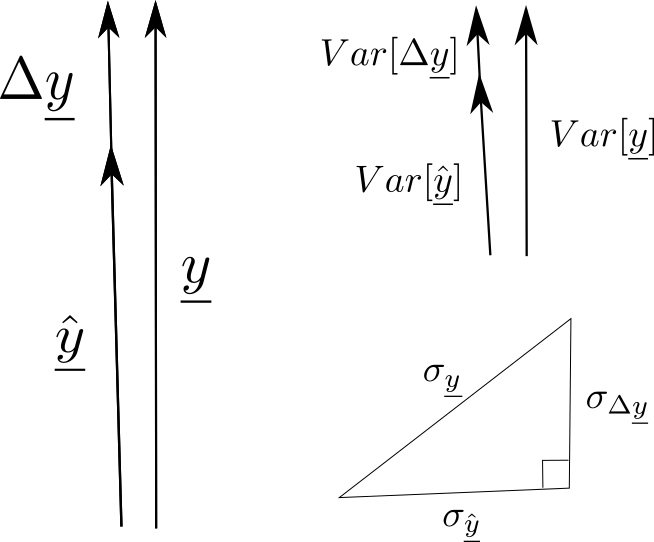
\includegraphics[width=2.3in]
{conventions/ms-error.png}
\caption{$\rvy=\HAT{y}+\Delta y$
and the variances (not standard deviations)
of these quantities add. }
\label{fig-ms-error}
\end{figure}

\section{Cramer-Rao Bound}

This discussion of the Cramer-Rao (CR) bound
is based on Ref.\cite{wiki-cramer-rao}.

Suppose $\rvx$ is a random variable with values $x\in val(\rvx)$
and $\theta\in\RR$ is a parameter.
For any function
$f_{\rvx,\theta}: val(\rvx)\times \RR\rarrow \RR$,
define

\beq
\av{f_{\rvx,\theta}} =\sum_x P(x|\theta)f_{x,\theta}
\eeq

\beq
\Delta f_{\rvx,\theta}=f_{\rvx,\theta}-\av{f_{\rvx,\theta}}
\eeq

\beq
\av{f_{\rvx,\theta},f_{\rvx,\theta}}=
\av{\Delta f_{\rvx,\theta}\;\Delta f_{\rvx,\theta}}
\eeq

Define the {\bf log likelihood function} by
\beq
LL_\theta = \ln P(x|\theta)
\eeq

Define the {\bf Fisher information} by
\beq
I_\theta=\av{\partial_\theta LL_\theta,\partial_\theta LL_\theta}
\eeq

Note that $LL_\theta\leq 0$.
Let $\theta^*$ be the
value of $\theta$ that maximizes $LL_\theta$.


Note that $I_\theta\geq 0$ and
$I_\theta=0$ when $\theta=\theta^*$
because $\partial_\theta LL_\theta|_{\theta=\theta^*}=0$.
This suggests that $I_\theta$
measures the distance
between $\theta$ and $\theta^*$.



Note that
\beqa
\av{\partial_\theta LL_\theta}&=&
\sum_x P(x|\theta)\frac{1}{P(x|\theta)}
\partial_\theta P(x|\theta)
\\
&=&
\partial_\theta \sum_x P(x|\theta)
\\
&=&
0
\eeqa
Therefore

\beqa
I_\theta &=&\av{[\partial_\theta LL_\theta]^2}
-
\av{\partial_\theta LL_\theta}^2
\\
&=&
\av{[\partial_\theta LL_\theta]^2}
\eeqa

\begin{claim}
\beq
I_\theta = -\av{\partial_\theta^2 LL_\theta}
\eeq
\end{claim}
\proof

\beqa
I_\theta &=& \av{[\partial_\theta LL_\theta]^2}
\\
&=&
\sum_x P(x|\theta)
\frac{1}{P(x|\theta)}
\partial_\theta P(x|\theta)
\partial_\theta \ln P(x|\theta)
\\
&=&
-\sum_x P(x|\theta)\partial_\theta^2 \ln P(x|\theta)
+ \partial_\theta\sum_x
P(x|\theta)\partial_\theta \ln P(x|\theta)
\\
&=&
-\av{\partial_\theta^2 LL_\theta}
+ \partial_\theta^2\sum_x P(x|\theta)
\\
&=&
-\av{\partial_\theta^2 LL_\theta}
\eeqa
\qed

\begin{claim}
If $x=[x_i]_{i=1,2, \ldots \nu}\in \RR^\nu$ are i.i.d., then


\beq
I_\theta = \nu \av{[\partial_\theta LL_{\theta, i}]^2}
\eeq
where

\beq
LL_{\theta, i} = \ln P(x_i|\theta)
\eeq
\end{claim}
\proof

\beqa
LL_\theta
&=& \ln \prod_i P(x_i|\theta)
\\
&=&
\sum_i LL_{\theta, i}
\eeqa

\beqa
I_\theta &=&
\sum_i \sum_j \av{
\partial_\theta LL_{\theta,i}
\partial_\theta LL_{\theta,j}
}
\\
&=&
\sum_i  \av{
[\partial_\theta LL_{\theta,i}]^2}
\\
&=&
\nu \av{
[\partial_\theta LL_{\theta,i}]^2
}
\eeqa
\qed




A function  $t_\rvx:val(\rvx)\rarrow \RR$
is called a {\bf test statistic} of random variable $\rvx$.

\begin{claim}(Cramer-Rao bound for single parameter $\theta\in\RR$)

\beq
\av{t_\rvx,t_\rvx}I_\theta \geq
 \left[\partial_\theta\av{t_\rvx}\right]^2
 \label{eq-crao-tx}
 \eeq
\end{claim}
\proof

Cauchy-Schwartz inequality

For two vectors $\veca,\vecb\in\RR^n$:
\beq
\veca\cdot\vecb =|\veca||\vecb|\cos \phi \leq |\veca||\vecb|
\eeq

For two real valued random variables $\rva, \rvb$:
\beq
\av{\rva, \rva} \av{\rvb,\rvb}\geq |\av{\rva,\rvb}|^2
\eeq
Replace

\beq
\rva\rarrow t_\rvx,
\quad\rvb\rarrow \partial_\theta LL_\theta
\eeq
Then

\beqa
\av{t_\rvx, \partial_\theta LL_\theta}
&=&
\av{t_\rvx \partial_\theta LL_\theta}
-
\av{t_\rvx} \underbrace{\av{\partial_\theta LL_\theta}}_{=0}
\\
&=&
\sum_x P(x|\theta)
t_\rvx \frac{1}{P(x|\theta)}\partial_\theta P(x|\theta)
\\
&=&
\partial_\theta\sum_x  t_\rvx P(x|\theta)
\\
&=&
\partial_\theta\av{ t_\rvx}
\eeqa
\qed

See Fig.\ref{fig-cramer-rao}
for a pictorial representation
of Eq.(\ref{eq-crao-tx}).

\begin{figure}[h!]
\centering
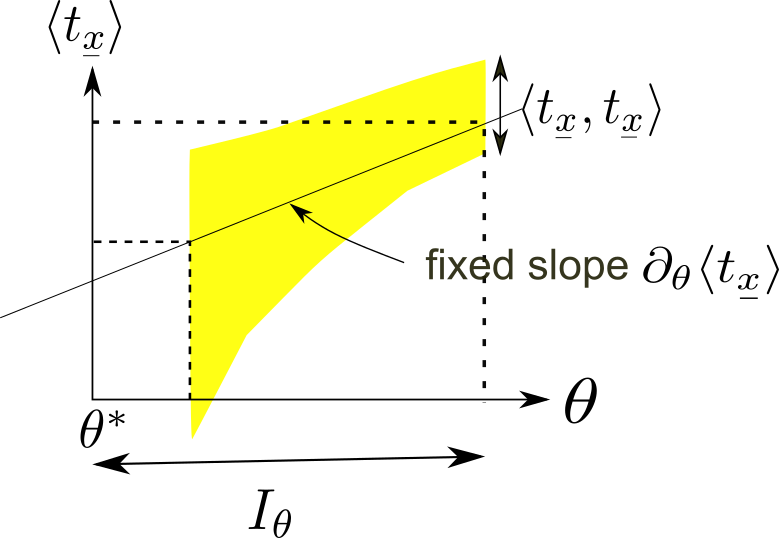
\includegraphics[width=2.7in]
{conventions/cramer-rao.png}
\caption{
In this drawing,
$\theta^*$ is the
value of $\theta$ that maximizes $LL_\theta$.
According
to the CR bound,
the product of the
variance $\av{t_\rvx, t_\rvx}$ and
the distance $I_\theta$
must be greater or equal to $[\partial_\theta\av{t_\rvx}]^2$.
At fixed $[\partial_\theta\av{t_\rvx}]^2$,
if the variance increases, the distance decreases,
and vice versa.
}
\label{fig-cramer-rao}
\end{figure}


Now suppose the test statistic $t_\rvx$
equals an {\bf estimator} $\HAT{\theta}$
of $\theta$ with bias $b_\rvx:val(\rvx) \rarrow \RR$.

\beq
t_\rvx = \HAT{\theta}(\rvx) = \theta + b_\rvx
\eeq
$\HAT{\theta}$ is said to be a {\bf biased estimator}
if $b_\rvx\neq 0$ and an {\bf unbiased estimator} if $b_\rvx=0$.

\begin{claim}

\beq
\av{\HAT{\theta}} = \theta + \av{b_\rvx}
\eeq

\beq
\av{\HAT{\theta}, \HAT{\theta}} \geq
\frac{[1 + \partial_\theta\av{b_\rvx}]^2}
{I_\theta}
\label{eq-crao-theta}
\eeq

\beq
\av{[\HAT{\theta}-\theta]^2} \geq
\frac{[1 + \partial_\theta\av{b_\rvx}]^2}
{I_\theta}
+
\av{b_\rvx}^2
\eeq

\end{claim}
\proof
\beqa
\partial_\theta\av{t_\rvx}
&=&
\partial_\theta\av{\theta + b_\rvx}
\\
&=&
\partial_\theta\left[\theta +\av{b_\rvx}\right]
\\
&=&
1 + \partial_\theta\av{b_\rvx}
\eeqa
Eq.(\ref{eq-crao-theta})
follows from Eq.(\ref{eq-crao-tx})
once we replace $t_\rvx$ by $\HAT{\theta}$.

Let
\beq
\Delta \HAT{\theta} =
\HAT{\theta} -\av{\HAT{\theta}}
=
\underbrace{(\HAT{\theta} -\theta)}_\xi  - \av{b_\rvx}
\eeq
Then

\beq
0=\av{\Delta \HAT{\theta}} = \av{\xi} - \av{b_\rvx}
\eeq

\beqa
\frac{[1 + \partial_\theta\av{b_\rvx}]^2}
{I_\theta} &\leq&
\av{[\Delta \HAT{\theta}]^2}
\\
&=&
\av{\xi^2 -2\xi\av{b_\rvx} + \av{b_\rvx}^2}
\\
&=&
\av{\xi^2} -\av{b_\rvx}^2
\eeqa

\qed

Multi-dimensional case:
parameter
 $\theta=[\theta_1, \theta_2, \ldots, \theta_n]^T\in \RR^n$
 and test statistic
 $t_\rvx=[t_{\rvx,1}, t_{\rvx,2}, \ldots, t_{\rvx,n}]^T\in \RR^n$
are column vectors.

Define {\bf Fisher information matrix} by

\beq
[I_\theta]_{i,j}=
\av{\partial_{\theta_i} LL_\theta, \partial_{\theta_j}LL_\theta}
=
\av{\partial_{\theta_i} LL_\theta\;\partial_{\theta_j}LL_\theta}
\eeq

CR bound for multi-dimensional parameter $\theta\in\RR^n$:
\beq
\text{matrix}\left[\av{t_{\rvx,i}, t_{\rvx,j}}\right]\geq
\text{matrix}\left[
\partial_{\theta_i} \av{t_{\rvx,a}}
[I_\theta]^{-1}_{a,b}
\partial_{\theta_j} \av{t_{\rvx,b}}
\right]
\eeq
where we are using the Einstein summation
convention (repeated indices are summed over).
For two matrices $A,B\in\RR^n$, $A\geq B$ means $A-B$ has
non-negative eigenvalues.


\section{Bayes Rule,
Bayesian Updating And Conjugate Priors}

Bayes Rule says:

\beq
P(\theta|x)P(x)
=
P(x|\theta)P(\theta)
\eeq
Expressed diagramatically\footnote{Two bnets are equated if their full probability
distributions (i.e.,
their full instantiations) are equal numerically.
For example,
$$
\rva\rarrow\rvb\rarrow \rvc = P(c|b)P(b|a)P(a)= \rva\larrow\rvb\larrow\rvc
$$},
we have for  $\rvx\in\RR$:
\beq
\xymatrix{
\rvtheta&\rvx\ar[l]
}
\quad =\quad
\xymatrix{
 \rvtheta\ar[r]&\rvx
}
\eeq
and for $\rvx=(\rvx_1, \rvx_2)\in \RR^2$:
\beq
\begin{array}{c}
\xymatrix@R=.3pc{
&\rvx_1\ar[ld]\ar[dd]
\\
\rvtheta
\\
&\rvx_2\ar[lu]
}
\xymatrix@R=.3pc{\\\quad =\quad}
\xymatrix@R=.3pc{
&\rvx_1\ar[dd]
\\
\rvtheta\ar[ru]\ar[rd]
\\
&\rvx_2
}
\end{array}
\eeq
Note how Bayes rule
allows us to reverse the
direction of the arrows
impinging on $\theta$.
We see from Bayes Rule
that even though
the directions of
the arrows in a
bnet can have causal
motivation, a bnet
with arrows reversed
from their causally
motivated directions
can still be very useful
as a calculation tool.

Another way of stating
Bayes Rule is




\beq
\underbrace{P(\theta|x)}_{\rm posterior}=
\caln(!\theta)
\underbrace{P(x|\theta)}_{\rm likelihood}
\underbrace{P(\theta)}_{\rm prior}
\;.
\eeq

If, for a given likelihood,
the prior and posterior
distributions belong to
the same family (for instance,
they are both
Beta distributions),
then we say that the prior is the
{\bf conjugate prior}
of that likelihood.

For example,
Beta $\sim$ Bernoulli*Beta.
Hence, the
Beta distribution\footnote{See
Ref.\cite{wiki-beta-dist} for a discussion
of the Beta distribution.}
is the conjugate prior of the
Bernoulli distribution\footnote{See
Ref.\cite{wiki-bern-dist} for a discussion
of the Bernoulli distribution}.
More explicitly,
if

\beq
p_1\sim {\rm Beta}(p_1;\alp, \beta)
\eeq
and

\beq
x|p_1\sim {\rm Bernoulli}(x;p_1)
\;,
\eeq
where $p_1=P(x=1)$,
then

\beq
p_1|x\sim {\rm Beta}(p_1;\alp', \beta')
\eeq
where

\beq
\alp'= \alp + x
\eeq

\beq
\beta'= \beta + (1-x)
\eeq


Ref.\cite{wiki-conj-prior}
has a table of
conjugate priors.

Conjugate priors facilitate
Bayesian updating
of the prior to
posterior in a
feedback loop(see Fig.\ref{fig-conj-prior}).

\begin{figure}[h!]
$$\xymatrix{
&x_t\ar[d]
\\
&\stackrel{Bernoulli}{P(x_t|\theta)}\ar@/_2pc/[ld]
\\
\stackrel{Beta}{P(\theta|x_{\leq t})}\ar@/_2pc/[rd]
&&\stackrel{Beta}{P(\theta|x_{\leq t-1})}\ar@/_2pc/[ul]
\\
&t\rarrow t+1 \text{ for } t=0, 1, 2,\ldots
\ar@/_2pc/[ur]
}$$
\caption{Bayesian updating facilitated
by conjugate prior. In this figure,
$x_{\leq t}=(x_0, x_1, \ldots, x_{t-1}, x_t)$.}
\label{fig-conj-prior}
\end{figure}



\section{Entropy,
 Kullback-Leibler divergence, Cross-Entropy}

For probability distributions $p(x), q(x)$ of $x\in val(\rvx)$
\begin{itemize}
\item
Entropy:
\beq
H(p)=-\sum_x p(x)\ln p(x)\geq 0
\eeq

\item
Kullback-Leibler divergence:

\beq
D_{KL}(p\parallel q)=\sum_{x} p(x)\ln \frac{p(x)}{q(x)}\geq 0
\eeq
\item
Cross entropy:
\beqa
CE(p\parallel q) &=& -\sum_x p(x)\ln q(x)\\
&=& H(p) + D_{KL}(p\parallel q)
\eeqa
\end{itemize}

\section{Definition of various
entropies used in Shannon Information Theory}
\label{sec-def-various-ents}

\begin{itemize}
\item
{\bf (plain) Entropy of $\rvx$}

\beq
H(\rvx) =
-\sum_{x} P(x)\ln P(x)
\eeq
This quantity measures the
spread of $P_\rvx$.
$H(\rvx)\geq 0$
and it vanishes iff $P(x)=\delta(x,x_0)$ (deterministic case)


\item
{\bf Conditional Entropy of $\rvy$ given $\rvx$}

\beqa
H(\rvy|\rvx) &=&
-\sum_{x,y}P(x,y)\ln {P(y|x)}
\\
&=&
H(\rvy,\rvx)-H(\rvx)
\eeqa
This quantity measures  the conditional
 spread
of $\rvy$ given $\rvx$. $H(\rvy|\rvx)\geq 0$.


\item {\bf Mutual Information (MI)
of $\rvx$ and $\rvy$}.

\beqa
H(\rvy:\rvx) &=&
\sum_{x,y} P(x,y) \ln \frac{P(x,y)}{P(x)P(y)}
\\
&=&
H(\rvx) + H(\rvy) - H(\rvy,\rvx)
\eeqa
This quantity measures the correlation
between $\rvx$ and $\rvy$.
$H(\rvy:\rvx)\geq 0$
and it vanishes iff
$P(x,y)=P(x)P(y)$.

\item {\bf Conditional Mutual Information
(CMI)\footnote{CMI
can be read as \qt{see me}.}
of $\rvx$ and $\rvy$
given $\ul{\lam}$}


\beqa
H(\rvy:\rvx|\ul{\lam})
&=&
\sum_{x,y, \lam}P(x,y, \lam) \ln
\frac{P(x,y|\lam)}{P(x|\lam)P(y|\lam)}
\\
&=&
H(\rvx|\ul{\lam}) + H(\rvy|\ul{\lam})
- H(\rvy,\rvx|\ul{\lam})
\eeqa

This
quantity measures the conditional correlation
of $\rvx$ and $\rvy$ given $\ul{\lam}$.
$H(\rvy:\rvx|\ul{\lam})\geq 0$
and it vanishes iff
$P(x,y|\lam)=P(x|\lam)P(y|\lam)$.

An interesting special case
occurs when
$P(\lam)=\delta(\lam, \lam_0)$ (the
frequentist  case of no $\lam$ prior.)
In that case CMI
reduces to

\beq
H(\rvy:\rvx|\lam_0)
=
\sum_{x,y}P(x,y|\lam_0) \ln
\frac{P(x,y|\lam_0)}{P(x|\lam_0)P(y|\lam_0)}\geq 0
\eeq



\item {\bf Kullback-Leibler Divergence
from $P_\rvx$ to $P_\rvy$.}

Assume random variables $\rvx$
and $\rvy$
have the same set of states
$val(\rvx)=val(\rvy)$. Then


\beq
D_{KL}(P_\rvx\parallel P_\rvy)=
\sum_x P_\rvx(x) \ln \frac{P_\rvx(x)}{P_\rvy(x)}
\eeq

This quantity measures a non-symmetric distance
between the probability distributions
$P_\rvx$ and $P_\rvy$.
$D_{KL}(P_\rvx\parallel P_\rvy)\geq 0$
and it equals zero iff $P_\rvx=P_\rvy$.

\end{itemize}

\section{Mean log likelihood asymptotic behavior}
\label{sec-ent-like-connect}

Define the log likelihood  by
\beq
 LL_{y|\theta} = \ln P(y|\theta)
\;.
\eeq
In this section, we will represent averages over $\rvy|\theta$ by
angular brackets:
\beq
\av{f(y)}= \sum_y P(y|\theta) f(y)= E_{\rvy|\theta}[f(y)]
\;.
\eeq
Note that the mean log likelihood equals minus the entropy:

\beq
H(\rvy|\theta)= -\av{ LL_{y|\theta}}
\eeq

\begin{claim}

\beq
\av{\partial_\theta   LL_{y|\theta}}=0
\eeq

\beq
\av{\partial^2_\theta   LL_{y|\theta}}=
-\av{ (\partial_\theta  LL_{y|\theta})^2 }
\eeq

\end{claim}
\proof

\beqa
\av{\partial_\theta   LL_{y|\theta}}
&=&
\sum_y P(y|\theta)\partial_\theta\ln  P(y|\theta)
\\
&=&
\sum_y \partial_\theta P(y|\theta)
\\
&=& 0
\eeqa


\beqa
\av{\partial^2_\theta   LL_{y|\theta}}
&=&
\sum_y  P(y|\theta)\partial_\theta \left[ \frac{1}{P(y|\theta)}
 \partial_\theta P(y|\theta) \right]
\\
&=&
- \sum_y  P(y|\theta)
\frac{1}{P(y|\theta)^2}[ \partial_\theta P(y|\theta)]^2
+  \underbrace{ \sum_y   \partial_\theta^2   P(y|\theta)}_{=0}
\\
&=&
-\sum_y  P(y|\theta)[ \partial_\theta \ln P(y|\theta)]^2
\\
&=&
-\av{ (\partial_\theta  LL_{y|\theta})^2 }
\eeqa
\qed

Define
\beq
\Delta \theta =  \theta' - \theta
\eeq
and

\beq
-\Delta H(\rvy|\theta)=
\Delta\av{  LL_{y|\theta}}
=
\av{  LL_{y|\theta'}}-
\av{  LL_{y|\theta}}
\;
\eeq
If we expand
$\av{  LL_{y|\theta'}}$ as a Taylor series
to second order
about the point $\theta'=\theta$,
we get


\beq
\av{  LL_{y|\theta'}}=
\av{  LL_{y|\theta}}
+
\Delta \theta
\underbrace{\av{ \partial_\theta LL_{y|\theta}}}_{=0}
+
\frac{(\Delta\theta)^2}{2}
\underbrace{\av{ \partial^2_\theta LL_{y|\theta}}}_
{-\av{ (\partial_\theta LL_{y|\theta})^2} }
+ \calo((\Delta\theta)^3)
\eeq

\beq
-\Delta H(\rvy|\theta)=\Delta\av{  LL_{y|\theta}}
=
-\;\frac{(\Delta\theta)^2}{2}
\av{ (\partial_\theta LL_{y|\theta})^2}
+ \calo((\Delta\theta)^3)
\eeq
Thus, $\theta'=\theta$ maximizes
the mean log likelihood $\av{  LL_{y|\theta}}$
(and minimizes the entropy $H(\rvy|\theta)$).

Note that
\beq
\Delta\av{  LL_{y|\theta}}
=
\av{\ln \frac{P(y|\theta')}{P(y|\theta)}}
\;.
\eeq
If we approximate
the ratio of these 2 probabilities by a Gaussian,

\beq
\frac{P(y|\theta')}{P(y|\theta)}
\approx \exp \left(-\;\frac{(\Delta \theta)^2}{2\s^2_\theta}\right)
\;,
\eeq
then

\beq
\s^2_\theta = \av{ (\partial_\theta LL_{y|\theta})^2}^{-1}
\;.
\eeq


\section{Arc Strength (Arc Force)}

Given a bnet with an arc (i.e., arrow) $\rvx\rarrow \rvy$,
we define the {\bf arc strength or arc force}
of arc $\rvx\rarrow \rvy$
to be
$H(\rvx:\rvy)$ (i.e., the mutual information between $\rvx$ and
$\rvy$). Evaluation of $H(\rvx:\rvy)$ requires knowing
$P(y|x)$, $P(x)$ and $P(y)$.
$P(y|x)$ is the TPM of node $\rvy$, so it is immediately
available from the specification of the bnet.
Calculating $P(x)$ and $P(y)$ is more involved,
and  requires marginalizing the full probability
distribution of the bnet. Such marginalizations can be
done using the junction tree algorithm described in
Chapter \ref{ch-junc-tree}.


\section{Pearson Chi-Squared Test}

The
{\bf Pearson divergence}
(a.k.a. {\bf Pearson Chi-squared test statistic})
for two
probability distributions
$PO(x)$ and $PE(x)$,
where $x\in val(\rvx)$,
is defined
as follows:
\beq
D_{\chi^2}=
\sum_x
\frac{[PO(x)-PE(x)]^2}{PE(x)}
=
\sum_x \frac{PO^2(x)}{PE(x)}-1
\;.
\eeq
Usually $PO$ is the
observed probability distribution and
$PE$ is the expected, theoretical one.

As the following claim shows,
the Pearson divergence
is closely related to the
Kullback-Leibler divergence.


\begin{claim}
If $\left|\frac{PO(x)}{PE(x)}-1\right|<<1$
for all $x\in val(\rvx)$, then

\beq
D_{KL}(PO\parallel PE)\approx D_{\chi^2}
\;.
\eeq
\end{claim}
\proof
\beqa
D_{KL}(PO\parallel PE)
&=&
\sum_x PO(x)\ln \frac{PO(x)}{PE(x)}
\\
&=&
\sum_x PO(x)\ln
\left(1 + \frac{PO(x)}{PE(x)} -1
\right)
\\
&\approx&
\sum_x
PO(x)\left(
\frac{PO(x)}{PE(x)} -1
\right)
\\
&=&
\sum_x
\frac{PO^2(x)}{PE(x)} -1
\\
&=&
D_{\chi^2}
\eeqa
\qed

Let $nx=|val(\rvx)|$.
Let $P_{\chi^2}(y)$
be the $\chi^2$
(with $nx-1$ degrees of freedom)
probability
distribution,
and let $F_{\chi^2}(\alp)$
be its cumulative
distribution.
Find $\alp$
such that
\beq
95\%=\int_{0}^{\alp}dy\; P_{\chi^2}(y)=
F_{\chi^2}(\alp)
\eeq
If $D_{\chi^2}<\alp$,
then we say that $PO=PE$ to 95\%
significance level (SL),
whereas if
$D_{\chi^2}>\alp$,
we say that $PO\neq PE$
to 95\% SL (i.e., SL$=95\%$).
The higher SL becomes,
the higher $\alp$ becomes,
and the bigger the
divergence $D_{\chi^2}$
has to be,
before we are
willing to declare that $PO\neq PE$.

\section{Demystifying Population
and Sample Variances}
Let $x[\s]=x^\s$.
Given  i.i.d.real  variables
$(x^\s)_{\s=0,1, \ldots, n-1}$,
let\footnote{Do not confuse the sample
index $\s$ and the standard deviation
$\s$.}

\beq
\HAT{\mu}=\ol{x}=
\frac{1}{n}
\sum_\s x^\s
\;
\eeq

\beq
(\hatvar)_\infty=
\frac{1}{n}
\sum_\s (x^\s-\mu)^2
\eeq

\beq
\hatvar=
\frac{1}{n-1}
\sum_\s (x^\s-\HAT{\mu})^2
\eeq

Statisticians\footnote{
In the language of Statisticians,
 a \qt{population}
is supposed to be
so large that its $\mu$
does not fluctuate,
and a \qt{sample} is
supposed to be a small
subset of that population
for which the $\mu$
is assumed to fluctuate.
In this book, I
use the word \qt{population}
to mean a set of any size
containing individuals, I use
the word \qt{sub-population}
to refer to a subset
of the population,
and I use the
word \qt{sample}
(a.k.a. individual, observation, unit,
record)  to mean a
single individual
of the population.} call
$(\hatvar)_\infty$ the
\qt{population variance}. I will
call it the {\bf population
variance for fixed $\mu$}.
Note that it depends
on
the fixed parameter $\mu$.
Statisticians   call
$\hatvar$ the
\qt{sample variance}.
Instead,
 I will
call $\hatvar$ the {\bf
population
variance for random $\mu$}.

If one treats $x^\s$ as a random
variable, then one must treat
$\HAT{\mu}$
as a random variable too.
Let
\beq
E[\rvx^\s]=\mu
\eeq
and

\beq
\av{\rvx^\s, \rvx^{\s'}}=
\delta(\s, \s')\s^2
\;.
\eeq
Then one can show that

\beqa
E[\ul{(\hatvar)_\infty}]
&=&
\frac{1}{n}
E\left[
\sum_\s (\rvx^\s-\mu)^2
\right]
\\
&=&
\s^2
\eeqa
and

\beqa
E[\ul{\hatvar}]
&=&
\frac{1}{n-1}
E\left[
\sum_\s (\rvx^\s-\HAT{\ul{\mu}})^2
\right]
\\
&=&
\s^2
\eeqa
This is the
reason
why
we use
an $n-1$
instead
of an $n$
in $\hatvar$.
Because it
makes
$E[\hatvar]=\s^2$
so
$\hatvar$
is an
unbiased estimator of
the single individual variance $\s^2$.

The intuitive reason for
why $\hatvar$
is divided
by $n-1$
instead of $n$
is that whereas $\mu$
in $(\hatvar)_\infty$
is kept fixed
and is \qt{quiet},
the $\ul{\HAT{\mu}}$
in  $\hatvar$
is a random variable,
noisy instead of quiet.
The fluctuations in
$\ul{\HAT{\mu}}$
are strongly
correlated with
the fluctuations
of the $\rvx^\s$,
so they decrease the
fluctuations  in $\hatvar$
compared to those in
$(\hatvar)_\infty$.
By dividing by $n-1$
instead of $n$,
we compensate for this
decrease in fluctuations
so that the ratio
of the numerator
and denominator
of  $\hatvar$
equals $\s^2$,
instead of something
{\it smaller} than $\s^2$,
as would happen if were to divide
by $n$ instead of $n-1$.
In terms of \qt{degrees of freedom}(DOFs),
$(\hatvar)_\infty$ has $n$ DOFs
(namely one for each $\rvx^\s$),
whereas $\hatvar$
has $n-1$ DOFs.
(the presence of $\ul{\HAT{\mu}}$
subtracts one DOF).
In both $(\hatvar)_\infty$
and $\hatvar$,
one divides by the number of DOFs.

\section{Independence of $\widehat{\mu}$
and $\widehat{\sigma^2}$} % hyperrefs can't take \HAT
\label{sec-ind-mu-sig-hat}

Let $x[\s]=x^\s$.
Consider i.i.d.real  variables
$(x^\s)_{\s=0,1, \ldots, n-1}$
such that\footnote{Do not confuse the sample
index $\s$ and the standard deviation
$\s$.}
\beq
E[\rvx^\s]=\mu
\eeq

\beq
\av{\rvx^\s, \rvx^{\s'}}=
\delta(\s, \s')\s^2
\;.
\eeq

\beq
\HAT{\mu}=\ol{x}=
\frac{1}{n}
\sum_\s x^\s
\;
\eeq

\beq
(\hatvar)_\infty=
\frac{1}{n}
\sum_\s (x^\s-\mu)^2
\eeq

\beq
\hatvar=
\frac{1}{n-1}
\sum_\s (x^\s-\HAT{\mu})^2
\eeq


\begin{claim}\label{claim-3Delta}
Let
\beq
\rvDel^\s= \rvx^\s-\mu
\;.
\eeq
For any $\s_1, \s_2, \s_3$,
\beq
\av{\rvDel^{\s_1}\rvDel^{\s_2}, \rvDel^{\s_3}}=0
\;.
\eeq
\end{claim}
\proof

Suppose $\s_2\neq\s_3$.
Then

\beq
\av{\rvDel^{\s_1}\rvDel^{\s_2}, \rvDel^{\s_3}}
=\underbrace{\av{\rvDel^{\s_2}}}_{0}
\av{\rvDel^{\s_1}, \rvDel^{\s_3}}
=0
\;.
\eeq
So assume $\s_2=\s_3=\s$
and evaluate
$\av{\rvDel^{\s_1}\rvDel^{\s}, \rvDel^{\s}}$.

Suppose $\s_1\neq \s$. Then
\beq
\av{\rvDel^{\s_1}\rvDel^{\s}, \rvDel^{\s}}=
\underbrace{\av{\rvDel^{\s_1}}}_{0}
\av{\rvDel^{\s}, \rvDel^{\s}}=0
\;.
\eeq
So suppose $\s_1=\s$ and evaluate
$\av{(\rvDel^{\s})^2, \rvDel^{\s}}$.

\beq
\av{(\rvDel^{\s})^2, \rvDel^{\s}}=
\underbrace{\av{(\rvDel^\s)^3}}_0
-\av{(\rvDel^\s)^2}
\underbrace{\av{\rvDel^\s}}_0=0
\;.
\eeq
\qed

\begin{claim}
\beq
\av{ \HAT{\ul{\s^2}}, \HAT{\rvmu}}=0
\;.
\eeq
\end{claim}
\proof
\beqa
\av{ \HAT{\ul{\s^2}}, \HAT{\rvmu}}
&=&\frac{1}{n(n-1)}
\sum_{\s, \s'}\av{
\left(\rvx^\s-\;\frac{1}{n}\sum_{\s''}\rvx^{\s''}\right)^2,
\rvx^{\s'}}
\\
&=&\frac{1}{n(n-1)}
\sum_{\s, \s'}\av{
\left(\rvx^\s-\;\frac{1}{n}\sum_{\s''}\rvx^{\s''}\right)^2,
\rvDel^{\s'}}
\\
&=&\frac{1}{n(n-1)}
\sum_{\s, \s'}\av{
\left(\rvDel^\s-\;\frac{1}{n}\sum_{\s''}\rvDel^{\s''}\right)^2,
\rvDel^{\s'}}
\\
&=&0\;\;\;\; \text{by Claim \ref{claim-3Delta}}
\;.
\eeqa
\qed

\section{Chi-square distribution}
This section
is based on Ref.\cite{wiki-chi-sq}.

\begin{figure}[h!]
$$
\xymatrix{
\rvq&\rvz.\ar[l]
}
$$
\caption{Bnet
used to define the Chi-square distribution.}
\label{fig-chi-sq}
\end{figure}

Let $q\in\RR$ and
$z.=\{z_i\}_{i=0,1, \ldots, \nu-1}$
where $z_i\in \RR$.
Consider the bnet of Fig.\ref{fig-chi-sq}.
The TPMs, printed in blue,
for that bnet, are as follows:\footnote{
Don't confuse the $q$
independent constant $\caln(!q)$
with the normal probability distribution
$\caln(x;\mu, \s^2)$.}




\beq
\color{blue}
P(z_i)=\caln(z_i; \mu=0, \s^2=1)
\;.
\eeq
We want
\beq
\rvq = \sum_{i=0}^{\nu-1} (\rvz_i)^2
\eeq
so $P(q|z.)$
is a Dirac delta function:

\beq
\color{blue}
P(q|z.)=\delta(
q - \sum_{i=0}^{\nu-1} (z_i)^2
)
\;.
\eeq
Therefore

\beqa
P(q) &=& \prod_{i=0}^{\nu-1}\left\{\int dz_i
\;P(z_i)
\right\}P(q|z_.)
\\
&=&
\caln(!q)q^{\frac{\nu}{2}-1}e^{-q/2}=\chi^2(q;\nu)
\;,
\eeqa
where $\caln(!q)$ is a constant that does not depend
on $q$ and is adjusted so that $\int_0^\infty dq\;P(q)=1$.

\section{Student's t-distribution}
This section
is based on Ref.\cite{wiki-stud}.

Let $x[\s]=x^\s$.
Consider i.i.d.real  variables
$(x^\s)_{\s=0,1, \ldots, n-1}$
such that\footnote{Do not confuse the sample
index $\s$ and the standard deviation
$\s$.}

\beq
E[\rvx^\s]=\mu
\eeq

\beq
\av{\rvx^\s, \rvx^{\s'}}=
\delta(\s, \s')\s^2
\;.
\eeq

\beq
\HAT{\mu}=\ol{x}=
\frac{1}{n}
\sum_\s x^\s
\;
\eeq

\beq
(\hatvar)_\infty=
\frac{1}{n}
\sum_\s (x^\s-\mu)^2
\eeq

\beq
\hatvar=
\frac{1}{n-1}
\sum_\s (x^\s-\HAT{\mu})^2
\;.
\eeq

If we define

\beq
z =
\frac{\HAT{\mu}-\mu}{\frac{\s}{\sqrt{n}}}
\label{eq-conv-zdef}
\;,
\eeq
then $\rvz$ has a Standard Normal
 Distribution (SND):

\beq
P(z)=\frac{1}{\sqrt{2\pi}}e^{-\;\frac{x^2}{2}}=\caln(z;\mu=0, \s^2=1)
\eeq
But what if we allow the standard deviation $\s$
to fluctuate in the expression
Eq.(\ref{eq-conv-zdef}) for $z$?
Define

\beq
t =
\frac{\HAT{\mu}-\mu}{\sqrt{\frac{\HAT{\s^2}}{n}}}
\;.
\label{eq-conv-tdef}
\eeq
Then one can show that
$\rvt$
has the {\bf Student's t-distribution}
${\rm Stud}(t;\nu=n-1)$
given by:

\beq
P(t)=
\caln(!t)
(1+\frac{t^2}{\nu})^{-\;\frac{\nu+1}{2}}=\text{Stud}(t;\nu=n-1)
\eeq

Note that if we use the approximation
$e^x\approx 1 +x +\calo(x^2)$,
we can show that ${\rm Stud}(t)$
tends to the SND
when $n>>1$:

\beqa
P(t)&=&\caln(!t)
(1+\frac{t^2}{\nu})^{-\;\frac{\nu+1}{2}}
\\
&\approx&
\caln(!t)e^{-\;\frac{t^2}{2}\frac{\nu+1}{\nu}}
\\
&\approx&
\caln(t; \mu=0, \s^2=1)
\;.
\eeqa

\hrule\noindent {\bf Partial derivation
of the explicit
form of ${\rm Stud}(t)$.}

Note that the $z$ definition
Eq.(\ref{eq-conv-zdef})
and the $t$ definition
Eq.(\ref{eq-conv-tdef}),
imply that
\beq
t= z
\underbrace{\sqrt{\frac{\s^2}{\HAT{\s^2}}}}_{\varrho}
\;,
\eeq
In the
expression $\rvt=\rvz\ul{\varrho}$,
the
 random variables
$\rvz$ and $\ul{\varrho}$
are independent
because, as shown in Section
\ref{sec-ind-mu-sig-hat},
 $\HAT{\mu}$
and $\HAT{\sigma^2}$
are independent.
Therefore, the random variable $\rvt$
can be defined using the bnet
of Fig.\ref{fig-stud-bnet}.

\begin{figure}[h!]
$$
\xymatrix{
&\ul{\varrho}\ar[ld]
\\
\rvt&\rvz\ar[l]
}
$$
\caption{Bnet used to define
the Student's t-distribution.}
\label{fig-stud-bnet}
\end{figure}
The TPMs, printed in blue,
for the bnet Fig.\ref{fig-stud-bnet},
are as follows:

\beq\color{blue}
P(t|z, \varrho)=
\delta(t- z\varrho)
\;\;\;\text{(Dirac delta function)}
\eeq

\beq\color{blue}
P(z)=\caln(z; \mu=0, \s^2=1)
\eeq

\beq\color{blue}
P(\varrho)=\text{given by
 Eq.(\ref{eq-stud-rho-pd}) below.}
\eeq

Note that
\beqa
P(\rvt=t)&=&
P(\rvz\ul{\varrho}=t)
\\
&=&
\int d\varrho\;
P(\rvz=\frac{t}{\varrho}|\varrho)P(\varrho)
\\
&=&\int d\varrho\;
\caln(\frac{t}{\varrho}; 0, 1)P(\varrho)
\\
&=&\int d\varrho\;
\frac{1}{\sqrt{2\pi}}
e^{-\;\frac{1}{2}(\frac{t}{\varrho})^2}P(\varrho)
\;.
\eeqa
If we define $q$ by

\beq
q =\frac{n-1}{\varrho^2}
\;,
\label{eq-stud-def1-q}
\eeq
then

\beq
q=\frac{(n-1)\hatvar}{\s^2}
=
\frac{1}{\s^2}
\sum_{\s=0}^{n-1}(x^\s-\HAT{\mu})^2
\;.
\label{eq-stud-def2-q}
\eeq
As a consequence of
\qt{Cochran's Theorem}
(see Ref.\cite{wiki-coch-theo}),
$\rvq$ given
by Eq.(\ref{eq-stud-def2-q}) must have
a Chi-square probability
distribution with $\nu=n-1$
degrees of freedom:\footnote{Note
that this $q$
is a quadratic form
$q=\vec{x}^T M \vec{x}$,
where $\vec{x}$ is an $n$ dimensional
column vector with components
$x^\s$,
and $M$ is an $n\times n$ matrix.
Cochran's Theorem
diagonalizes $M$
and replaces the
vectors $\vec{x}$
by equivalent ones in a new
basis.
Then the number
of $DOF$s (degrees of freedom)
of the chi-square distribution
is the number of non-zero
diagonal elements in
 the diagonalized $M$
(this
number is called the rank of $M$).
In the particular case of
Eq.(\ref{eq-stud-def2-q}),
$DOF=n-1$.}

\beq
P(q)= \chi^2(q;\nu=n-1)
\eeq

Henceforth, let $\nu=n-1$.
From the definition
Eq.(\ref{eq-stud-def1-q})
of $q$, we get

\beq
dq=
\frac{-2\nu}{\varrho^3}d\varrho
\;.
\eeq
Therefore,


\beqa
P(\varrho)d\varrho
&=&
P(q)dq
\\
&=&
\chi^2(\frac{\nu}{\varrho^2};\nu)\frac{(-2\nu)}{\varrho^3}d\varrho
\\
&=&
\caln(!\varrho)
\left(\frac{\nu}{\varrho^2}\right)
^{\frac{\nu}{2}-1}e^{-\;\frac{\nu}{2\varrho^2}}
\frac{d\varrho}{\varrho^3}
\\
&=&\caln(!\varrho)
\frac{d\varrho}
{\varrho^{\nu+1}}e^{-\;\frac{\nu}{2\varrho^2}}
\;.
\label{eq-stud-rho-pd}
\eeqa
Hence,

\beqa
P(t)&=&\caln(!t)
\int_0^\infty
\frac{d\varrho}
{\varrho^{\nu+1}}e^{-\;\frac{\nu}{2\varrho^2}}
e^{-\;\frac{1}{2}(\frac{t}{\varrho})^2}
\\
&=&\caln(!t)
\int_0^\infty
\frac{d\varrho}
{\varrho^{\nu+1}}
e^{-\;\frac{1}{2}\frac{t^2+\nu}{\varrho^2}}
\;.
\eeqa

\section{Hypothesis testing and 3 classic test statistics
(Likelihood, Score, Wald)}

Suppose we have
data $\vec{x}=[x^\s]_{\s=0, 1, \ldots,
nsam-1}$ which is distributed
according to
a probability distribution
$P(\vec{x};\theta)$
which depends
on some parameters $\theta=
(\theta_i)_{i=0, 1, \ldots,n-1}\in \RR^n$.
We define the
\begin{itemize}
\item
{\bf Likelihood of $\theta$} by

\beq
L(\theta)=P(\vec{x}|\theta)
\;,
\eeq
\item
the {\bf Maximum Likelihood estimate
of $\theta$} by

\beq
\HAT{\theta}=\argmax_\theta L(\theta)
\;,
\eeq
\item
the
{\bf log likelihood of $\theta$} by

\beq
LL(\theta) =\ln L(\theta)
\;,
\eeq
\item
the {\bf Score} or {\bf Lagrange
Multiplier vector}\footnote{$sc_i(\theta)=
\partial_{\theta_i}LL(\theta)$
is called a Lagrange multiplier
because to maximize $LL(\theta)$
over $\theta$ subject to
the constraint $\theta=\theta^*$,
we maximize
the Lagrangian $\call= LL(\theta)
-\sum_i \alp_i[\theta_i - \theta^*_i]$ over
$(\theta_i,\alp_i)$ for all $i$. The latter
gives $\alp_i=\partial_{\theta_i}LL(\theta^*)$
and $\theta=\theta^*$.
For a general
constrained optimization
problem, $\call=LL(\theta)-\sum_i \alp_ic_i(\theta)$
for some constraint functions $c_i(\theta)$.
Hence, $\alp_i=\partial_{\theta_i}LL/
\partial_{\theta_i}c_i$
and $c_i(\theta)=0$
for all $i$.
So, in general,
a Lagrange multiplier
is a ratio of two partial
derivatives.} of $\theta$ by

\beq
sc(\theta)=[sc_i(\theta)]\in \RR^n
\;,
\eeq
where

\beq
sc_i(\theta)=\partial_{\theta_i}LL(\theta)
\;,
\eeq
\item
and the
{\bf Fisher Information Matrix
of $\theta$} by

\beq
FI(\theta)= [FI_{i,j}(\theta)]\in \RR^{n\times n}
\eeq
where
\beq
FI_{i,j}(\theta)
=-
E_{\vec{\rvx}|\theta}
[
\partial_{\theta_i}\partial_{\theta_j}
\overbrace{
\ln P(\vec{\rvx}|\theta)}^{LL(\theta)}
]
\;.
\eeq
\end{itemize}

Note that if

\beq
LL(\theta)=\ln P(x|\theta)=
 \frac{-(\theta
-\HAT{\theta})^2}{2\s^2} + \caln(!\theta)
\;,
\label{eq-normal-ll}
\eeq
then

\beq
sc(\theta)=\frac{-(\theta-\HAT{\theta})}{\s^2}
\eeq
and

\beq
FI(\theta)=\frac{1}{\s^2}
\eeq



In hypothesis testing, one has
 a {\bf null hypothesis}
$H_0$: $\theta=\theta^*$,
and an {\bf alternative hypothesis}
 $H_1$: $\theta\neq \theta^*$.
We use a {\bf test statistic}
$\lam(\theta^*, \HAT{\theta})\geq 0$
which
measures a kind of
distance or separation between the
estimate $\HAT{\theta}$
and
the value $\theta^*$
for the null Hypothesis $H_0$.
For some {\bf confidence level} $C>0$,
if $\lam(\theta^*, \HAT{\theta})> C$,
$H_0$ is {\bf rejected}, whereas
if $\lam(\theta^*, \HAT{\theta})\leq C$,
$H_0$ is {\bf accepted}.


$\alp=1-C$ is called the
{\bf significance level}.
Usually $\alp<<1$
represents
the area under both
tails
of a Normal
distribution,
 and $C\approx 1$
represents
all the area except the tails of a
Normal distribution.

\begin{figure}[h!]
\centering
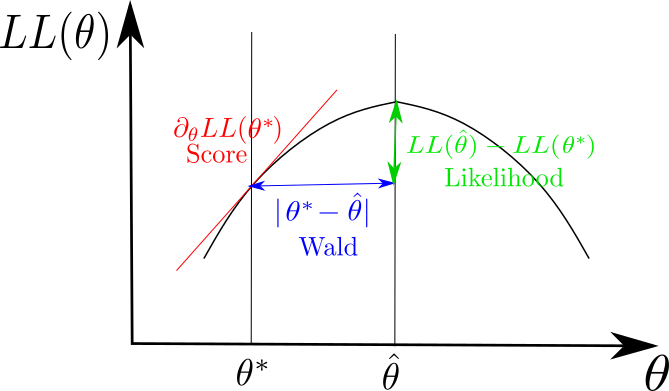
\includegraphics[width=3.2in]{conventions/classic-trio.png}
\caption{For $n=1$ and $\theta\in\RR$,
this figure shows the geometrical significance of
certain
quantities that
characterize the
3 classic test statistics
(Likelihood, Score, Wald)
for hypothesis testing.}
\label{fig-classic-trio}
\end{figure}

Henceforth in this section,
we will
occasionally  use the
Einstein summation
convention; i.e., implicit sum over
repeated indices.

Three classic test statistics
are (See Fig.\ref{fig-classic-trio}):

\begin{enumerate}

\item
{\bf Likelihood Ratio test statistic}
(Ref.\cite{wiki-Li-test}.)

\beq
\lam_{Li}=
2\ln\left[
\frac{L(\HAT{\theta})}
{L(\theta^*)}
\right]=
2[LL(\HAT{\theta})-LL(\theta^*)]
\eeq

\item
{\bf Score (a.k.a.
Lagrange multiplier) test statistic}
(Ref.\cite{wiki-Sc-test}.)

\beqa
\lam_{Sc}&=&
\partial_{\theta_i} LL(\theta^*)
\left[
FI(\theta^*)^{-1}\right]_{i,j}
\partial_{\theta_j} LL(\theta^*)
\\
&=&
\frac{[\partial_\theta LL(\theta^*)]^2}
{FI(\theta^*)}\quad \text{if $n=1$}
\eeqa
Doesn't depend on $\HAT{\theta}$.

\item
{\bf Wald test statistic}
(Ref.\cite{wiki-Wa-test}.)


\beqa
\lam_{Wa}&=&
(\HAT{\theta}-\theta^*)_i
\left[
\av{\HAT{\rvtheta},\HAT{\rvtheta}^T}^{-1}
\right]_{i,j}
(\HAT{\theta}-\theta^*)_j
\label{eq-wald-stat}
\\
&=&
\frac{(\theta^*-\HAT{\theta})^2}
{\av{\HAT{\theta},\HAT{\theta}}}
\quad\text{if $n=1$}
\eeqa

More generally,
one can replace $\theta^*\rarrow R\theta^*$
and  $\HAT{\theta}\rarrow R\HAT{\theta}$
in Eq.(\ref{eq-wald-stat}),
where $\theta^*$ and
$\HAT{\theta}$ are $n$ dimensional
column vectors, and
$R\in\RR^{\nu\times n}$.
The null and alternative hypotheses become:
$H_0: R\theta=R\theta^*$
and $H_1: R\theta\neq R\theta^*$.
Note that
$\nu$
is the number of
constraints imposed by the
null hypothesis. $R$ is called a
reparametrization of $\theta$.
The Wald test is not
reparametrization
invariant (i.e., $R$
invariant), but the Likelihood Ratio test is.

\end{enumerate}

Note that
if $LL(\theta)$
is given by Eq.(\ref{eq-normal-ll}),
then
$\av{\HAT{\rvtheta},\HAT{\rvtheta}}
=
\s^2=\frac{1}{FI(\theta)}
$. Hence,

\beq
\lam_{Li}=\lam_{Sc}=\lam_{Wa}=
\frac{(\HAT{\theta}-\theta^*)^2}{\s^2}
\eeq

Many
other commonly used test statistics
(or their squares)
are special cases of one
of the 3 classic test statistics.
For example, the z-statistic
used with normal
distributions,
the t-statistic
used with the
Student t-distribution,
the F-statistic used in linear regression,
the chi-squared statistic used
to do Pearson's chi-squared test.

{\bf Asymptotic Behavior}

If the data
$\vec{x}$ is i.i.d.,

\beq
P(\vec{x}|\theta)=
\prod_{\s=0}^{nsam-1} P(x^\s|\theta)
\;
\eeq
Hence, as $nsam\rarrow \infty$,

\beqa
LL(\theta)
&=&
\ln P(\vec{x}|\theta)
\\
&=&\sum_\s \ln
P(x^\s|\theta)
\\
&\rarrow&
nsam \sum_x P(x|\theta)\ln  P(x|\theta)
\\
&=&
-nsam \; H(\rvx|\theta)
\eeqa
Thus, {\it maximizing} the log likehood
$LL(\theta)$
and {\it minimizing} the entropy
$H(\rvx|\theta)$
give the same estimate $\HAT{\theta}$.

When the
data is i.i.d. and
$nsam\rarrow \infty$,
it is also possible to
prove that
the 3 test statistics
defined above all tend to
the same
probability  distribution, namely
$\calx^2(\theta^*; \nu)$,
the chi-square distribution
with $\nu$ degrees of freedom,
where $\theta\in \RR^n$, $R\in \RR^
{\nu\times n}$, and $\nu=n$ if $R=1$.

\section{Error Bars}
Never report measurements without error bars!!

Assume a distribution
with mean $\mu$ and
standard deviation $\s$
for a subpopulation with $n$
samples.

$SE=\frac{\s}{\sqrt{n}}$
is called the {\bf standard error}.


Some popular types of error bars:


\begin{itemize}
\item{\bf Box and Whiskers plot (a.k.a. Boxplot)}

See Fig.\ref{fig-boxplot}.
$IQR$ stands for {\bf
Intermediate Quantile Range}.
Sometimes, the endpoints of the
error bars are taken to be the minimum and maximum samples
instead of $Q_1- 1.5 *IQR$ and $Q_3+ 1.5 *IQR$.
The points that fall
in the intervals $[\min,Q_1- 1.5* IQR]$
and $[Q_3+ 1.5 *IQR, \max]$
are
called {\bf outliers}.
\begin{figure}[h!]
\centering
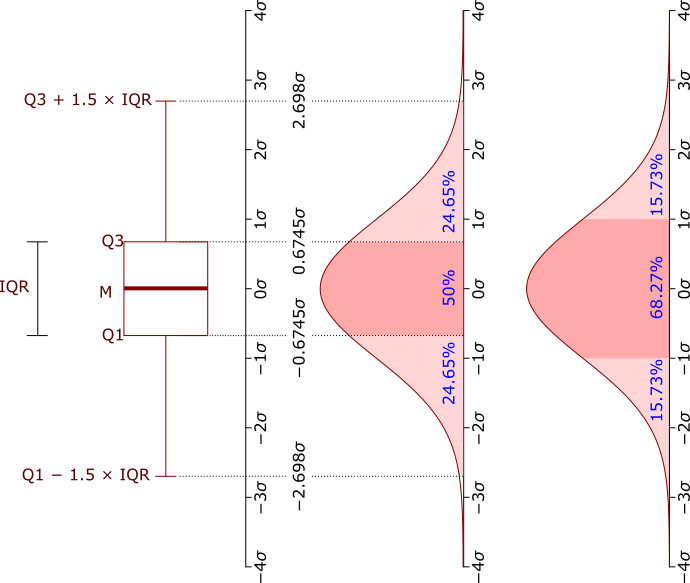
\includegraphics[width=3.3in]
{conventions/Boxplot.png}
\caption{Boxplot plot for Normal
distribution $\caln(\mu=0,\s)$.
$Q_1$ and $Q_3$ are the first and third
quantiles, and $M$ is the median (i.e., half-way point).
For a non-normal skewed
distribution, $Q_1$ and $Q_3$
are not equidistant from the median, and the
median is not exactly equal to the mean. }
 \label{fig-boxplot}
\end{figure}



\item{\bf Standard Deviation}

Error bar endpoints are located one standard deviation
away from the mean.
\beq
\mu-\s< \mu < \mu+\s
\eeq

\item{\bf Confidence Interval}

\beq
\mu-|z^*|SE <\mu < \mu+|z^*|SE
\label{eq-conf-int}
\eeq

$|z^*|=1.96$ for a confidence level of $95\%$.

The origin of Eq.(\ref{eq-conf-int})
is explained in the next section entitled \qt{Confidence Intervals}.
Confidence intervals are
derived from the Gaussian in Fig.\ref{fig-conf-int},
which should not be confused with the
Gaussian of Fig.\ref{fig-boxplot}.
They are different!

\end{itemize}
\section{Confidence Interval}

Normal distribution
with mean $\mu$
and standard deviation $\sigma$:

\beq
\caln(x;\mu, \s^2)=
\frac{1}{\s\sqrt{2\pi}}
e^{-\;\frac{(x-\mu)^2}{2\sigma^2}}
\;.
\eeq

Standard Normal Distribution (SND):
\beq
P(z)=\caln(z;0,1)
\eeq
Cumulative distribution for $P(z)$:

\beq
\Phi(z)=\int_{-\infty}^z dz'\;P(z')
\;.
\eeq

\begin{figure}[h!]
\centering
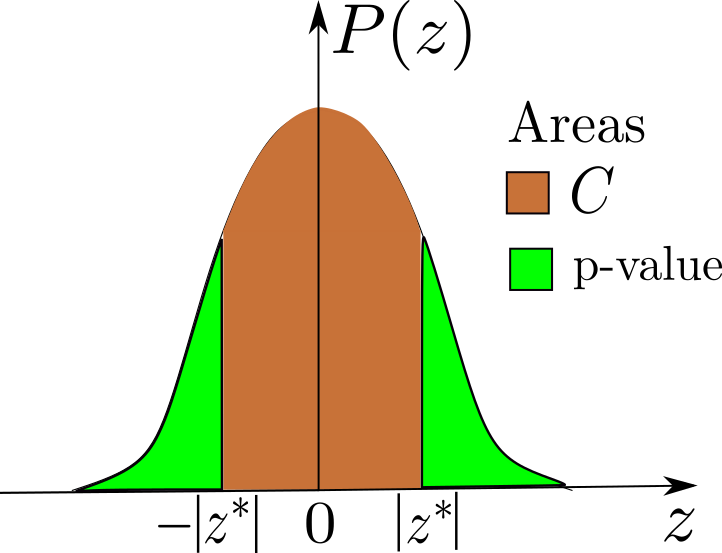
\includegraphics[width=2in]
{conventions/conf-int.png}
\caption{
Interpretation
of confidence level $C$
and p-value as areas under curve of the
Standard Normal Distribution (SND).}
\label{fig-conf-int}
\end{figure}

{\bf Confidence Level} $C$
and corresponding {\bf $|z^*|$ value}
(see Fig.\ref{fig-conf-int}):

\beq
C=\int_{-|z^*|}^{|z^*|} dz\;P(z) =
\Phi(|z^*|)-\Phi(-|z^*|)
=
2\left(\Phi(|z^*|)-\;\frac{1}{2}\right)
\label{eq-conf-level1}
\eeq
Equivalent definition:

\beq
C=P\left(
\underbrace{
\frac{|\rvx-\mu|}{\frac{\sigma}{\sqrt{n}}}
}_{|\rvz|}
<|z^*|\right)
\label{eq-conf-level2}
\eeq
For $C=95\%$,
$|z^*|=1.960\approx 2$.
For $C=99\%$, $|z^*|=2.576$.

Area of each tail
in Fig.\ref{fig-conf-int} is
usually called $\alpha$,
and the area of both tails is called
the {\bf p-value}:
\beq
C+\underbrace{2\alpha}_{p-value}=1
\;.
\eeq

Estimators\footnote{Don't
confuse the sample index $\s$
with the standard deviation $\s$.} of
mean $\mu$  and
standard deviation $\sigma$
from measurements $x^\s$
of a sub-population $\Sigma_1$ of
size $n=|\Sigma_1|$:
\beq
\HAT{\mu}=\ol{x}=\frac{1}{n}\sum_{\s \in\Sigma_1} x^\s
\eeq

\beq
\HAT{\s}^2=
\frac{1}{n-1}
\sum_{\s\in \Sigma_1} (x^\s-\ol{x})^2
\eeq


We get
from Eq.(\ref{eq-conf-level2}),
the {\bf Error bars (a.k.a. confidence intervals)}
and
{\bf Error $E$ (a.k.a. margin of error)}:



\beq
\text{ estimate of $x$
with error bars} =
\ol{x} \pm
\underbrace{
|z^*| \frac{\HAT{\s}}{\sqrt{n}}}_{E}
\label{eq-err-bars}
\eeq

\beq
n= \left(
\frac{|z^*|\HAT{\s}}{E}
\right)^2
\eeq

So far, we have assumed
that the sub-population (a.k.a. sample
population)
is normally distributed.
This might be false
for several reasons.
Some red flags: (1)
$n$ is too small (according to
a rule of thumb derived from
Central Limit Theorem, $n$
should be larger than 30
to insure a Normal Distribution).
(2) Sub-population not truly random
(i.i.d.)
because was taken
without replacement.
In many cases,
especially
when $n<30$,
the Student's t-distribution
models the sub-population statistics
much
better than the Normal distribution.


The {\rm Student's t-distribution } ${\rm Stud}(t;
\nu=n-1)$,
depends
on a parameter $\nu$
called the
number of
degrees of freedom.
In the case being considered here,
$\nu$ equals the
sub-population size $n$
minus one.
When fitting
the data with
Stud(), variable
$t$ replaces
variable $z$,
and ${\rm Stud}(t; \nu=n-1)$
replaces the Standard Normal distribution (SND)
$\caln(z; \mu=0, \sigma=1)$.
Stud() is symmetric about
the origin like SND,
but its tails
are fatter.
When fitting the data with Stud(),
the $|z^*|$
value is replaced
by a $|t^*|$ value.
Eq.(\ref{eq-conf-level1})
is replaced by


\beq
C=\int_{-|t^*|}^{|t^*|} dt\;{\rm Stud}(t) =
\Phi_S(|t^*|)-\Phi_S(-|t^*|)
=
2\left(\Phi_S(|t^*|)-\;\frac{1}{2}\right)
\label{eq-conf-level1-stu}
\;,
\eeq
where $\Phi_S()$
is the cumulative
distribution for  Stud().
Also, Eq.(\ref{eq-err-bars})
is replaced  by

\beq
\text{estimate of $x$
with error bars} =
\ol{x} \pm
\underbrace{
|t^*| \frac{\HAT{\s}}{\sqrt{n}}}_{E}
\;.
\eeq
Tables of $|t^*|(C,\nu=n-1)$
are available. Note
that $|t^*|$
depends on both $C$ and $\nu$,
whereas $|z^*|(C)$
depends only on $C$.

\section{Score p-value}
\label{sec-score-p-value}
When defining error bars
and confidence intervals in
Fig.\ref{fig-conf-int},
we defined a triplet
of values $(z, C, p)$
where $C+p=1$.
In this section,
we will consider a different triplet
of those values.
We will refer to the triplet
$(z_{th}, C_{th}, p_{th})$
used in error bars as the {\bf threshold triplet}, and to
the triplet
$(z_{sc}, C_{sc}, p_{sc})$
introduced in this section as the
{\bf score triplet}.
When we do hypothesis testing,
if $|z_{sc}|> |z_{th}|$
(i.e., if $z_{sc}$
falls outside
the error bars),
we say that the null
hypothesis is violated.
Equivalently, we say the null
hypothesis is violated
if $p_{sc}<p_{th}=1-C_{th}=0.05 \text{ typically}$.
Most statistics
books do a poor job
at distinguishing between
the threshold and score
triplets, and
seldom use distinguishing
subscripts like $th$ and $sc$.
In this book,
we will often
drop the $sc$
subscripts, but we will
try not to drop the $th$ subscripts.
Often, instead of
a $th$
subscript, we will
use an asterisk superscript.
For instance, instead
of $z_{th}$,
we might use $z^*$.
W\label{key}hen statisticians
use the term
\qt{p-value},
they are usually referring to
the score p-value,
although not always.



Given a parameter $\theta$, call
$\theta=\theta_0$ (or  $\theta<\theta_0$ or $\theta>\theta_0$) the
{\bf null hypothesis} $h_0$,
and call the negation of $h_0$ (i.e.,
$\theta\neq\theta_0$ (or  $\theta\geq\theta_0$ or $\theta\leq \theta_0$))
the {\bf alternative or
opposite hypothesis} $h_1$.
Assume we
are given data $\vec{x}=\{x^\s|\s\in \Sigma\}$. Assume
also that we are given
distributions $P(\rvx=x|h)$ for $h\in \{h_0, h_1\}$,
and $P(\rvx=x)$. Now let

\beq
P(\vec{x}|h)=\prod_\s P(\rvx=x^\s|h)
\eeq


\beq
P(\vec{x})=\prod_\s P(\rvx=x^\s)
\eeq
(so the $x^\s$ are i.i.d.).

A Bayesian would assume that there
is a prior $P(h)$, and use it to
calculate
$P(h|\vec{x})=\frac{P(\vec{x}|h) P(h)}{P(\vec{x})}$.
$P(\rvh= h_0|\vec{x})$
is the probability that the null hypothesis is true.
A p-value is a monotonically increasing function of
$P(\rvh= h_0|\vec{x})$,
so Bayesians have no trouble saying
that  {\color{red} a  p-value is
a measure of
$P(\rvh= h_0|\vec{x})$, i.e.,
a measure of the probability that
the null-hypothesis is true}.

Frequentists, on the other hand,
believe that $h$
is a \qt{parameter} which has an priori value; therefore,
it's not a random variable,
so  $P(\rvh= h_0|\vec{x})$
is undefined. To
circumvent this objection, a frequentist
would conduct a bunch of experiments
to decide whether $h$ equals $h_0$
or $h_1$. Then he/she
would say the p-value
is the fraction
of those experiments that claim $h=h_0$.

Next, we explain in more detail the correct
way of thinking about p-values, according to
Frequentists.
p-values were invented by Frequentists,
so it's worth hearing what they have to say
about them.
The Frequentist definition is not against Bayesianism,
and Bayesians, unlike Frequentists,
 don't accuse Frequentists of
having a sinfully incorrect
 definition of p-values. A Bayesian would just say:
our definition of p-values (shown
in red above) is not incorrect,
but the Frequentist definition is more precise than ours,
and doesn't assume a particular form for a prior.
We welcome it.

Call
the random variable
$\rvt$ the {\bf test or score statistic} and let
$t^*$ be a user defined
parameter.
$\rvt$ and $t^*$
are defined so that
when $\rvt=t^*$,
the $h_0$ hypothesis is
on the threshold between
being and not being satisfied.
Frequentists define the {\bf  p-value} $p$ as

\beq
p=
\left\{
\begin{array}{ll}
P(\rvt \geq t^*|h_0)&\text{right-sided-tail,
if $h_0$ is $\theta<\theta_0$}
 \\
 P(\rvt\leq t^*|h_0)&\text{left-sided-tail,
 if $h_0$ is $\theta>\theta_0$}
 \\
 P(|\rvt| > |t^*|\;|h_0)&\text{double-sided-tail,
 if $h_0$ is $\theta=\theta_0$}
\end{array}
\right.
\eeq
Thus, for a Frequentist,
{\color{red} a  p-value is a probabilistic
weight of the region
where the $h_0$ hypothesis is
defined (by the user) to be violated}.
If that weight is large,
then the region where
the $h_0$ hypothesis is
defined to be satisfied is small,
which means the $h_0$
hypothesis
is expected to be close to the truth.
The larger the p-value,
the closer $h_0$
is expected to be near the truth,
just like the Bayesian definition
says.
Note that the p-value
is a probability so it ranges in
value from 0 to 1.

Suppose we are given a sub-population with $n$ samples,
 mean $\ol{x}$ and variance $\HAT{\s}$.
 Let $\theta_0=\mu_0$.
Define

\beq
\rvt=\rvz=
\frac{\rvx-\mu_0}{\frac{\HAT{\s}}{\sqrt{n}}}
\;.
\eeq
For $n>30$,

\begin{subequations}
\beqa
P(\rvz\geq z^*|h_0)
=1-\Phi(z^*)=\Phi(-z^*)
&\quad&\text{if $h_0$ is $\mu<\mu_0$}
\\
P(\rvz\leq z^*|h_0)=\Phi(z^*)
&\quad&\text{if $h_0$ is $\mu>\mu_0$}
\\
P(|\rvz|\geq |z^*|\;|h_0)=2\Phi(-|z^*|)
&\quad&\text{if $h_0$ is $\mu=\mu_0$}
\label{eq-double-tail}
\eeqa
\end{subequations}
where $\Phi(x)$ is the cumulative distribution
for the Standard Normal Distribution
$\caln(x;\mu=0, \s=0)$.
For $n<30$, $\Phi()$ is replaced
by $\Phi_S()$, where  $\Phi_S()$ is
the cumulative distribution
for the Student t-distribution ${\rm Stud}(x; \nu=n-1)$.
Note that Eq.(\ref{eq-double-tail})
agrees with
Eq.(\ref{eq-conf-level2}).

The quantity
\beq
\hat{z}_{sc}=
\frac{\ol{x}-\mu_0}{\frac{\HAT{\s}}{\sqrt{n}}}
\eeq
is called the {\bf z score estimator}.
If $|\hat{z}_{sc}| > |z^*|$,
then the $h_0$ hypothesis
is defined to be violated
(for the double sided case).






\section{Convex/Concave functions,
Jensen's Inequality}
\label{sec-jensens}
Suppose $f:\RR\rarrow \RR$.
$f(x)$ is
a  {\bf concave function}
if
looks
like a cave ($\cap$) (i.e., $f''(x)>0$
if differentiable)
and it's a {\bf convex function} if it
looks like a valley ($\cup$)
(i.e., $f''(x)<0$
if differentiable).
More generally, if $f:\RR^a\rarrow \RR$,
$f(x)$ is said
to be concave
if $f(\alp x+\beta y)\geq \alp f(x)
+\beta f(y)$
and convex
if
$f(\alp x+\beta y)\leq \alp f(x)
+\beta f(y)$
for $\alp, \beta\in\RR$ and $x,y\in\RR^a$.

\begin{figure}[h!]
\centering
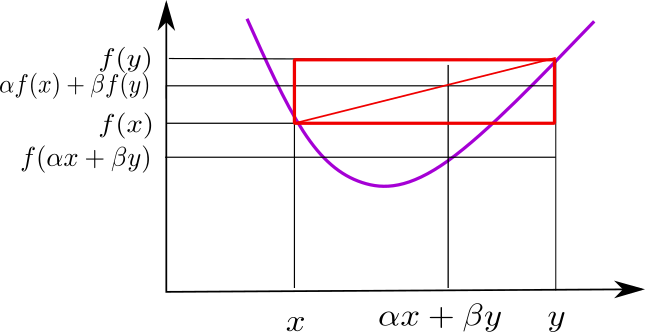
\includegraphics[width=4in]
{conventions/jensens.png}
\caption{Jensen's
inequality for sum of 2 terms, when
$f:\RR\rarrow\RR$ is
convex.}
\label{fig-jensens}
\end{figure}

Suppose $f:\RR^a\rarrow \RR$
is a convex function. Let
 $\alp,\beta$ be non-negative
 numbers that sum to 1,
 and $x,y\in \RR^a$.
From the definition of convexity,
 it follows that
(see Fig.\ref{fig-jensens}
for a geometrical
representation of this
when $a=1$)


\beq
f(\alp x + \beta y) \leq \alp f(x)
+ \beta f(y)
\eeq
{\bf Jensen's inequality} is
a simple generalization of this
inequality
to sums of more than 2 terms.
Let $\{p_i\}_{i=0}^n$ be
non-negative numbers that sum to one.
Also assume that
 $\{x_i\}_{i=0}^n$ are  elements of $\RR^a$.
Then

\beq
f\left(\sum_{=1}^n p_i x_i\right)
\leq
\sum_{=1}^np_i f(x_i)
\eeq
or, written in terms
of expected values,

\beq
f(E[\rvx])\leq E[f(\rvx)]
\eeq
The same result is true
if $f$ is concave
instead of convex and
we reverse the inequality
signs.

\section{Chebyshev's inequality}

Chebyshev's inequality (CI)
gives an upper bound for the area under the
2 tails (left and right ones)
of a probability distribution.

Below, we follow the
common practice of
proving CI
as a corollary of
Markov's Inequality (MI).


\begin{claim}(Markov's Inequality)
Let $\rvx$ be a non-negative random variable
and let $ a> 0$. Then

\beq
P(\rvx\geq a) \leq \frac{E[\rvx]}{a}
\eeq
\end{claim}
\proof
\beqa
\frac{E[\rvx]}{a}&=&
\frac{\int_0^\infty dx\; x P(x)}
{a}
\\
&\geq&
\frac{\int_a^\infty dx\; x P(x)}
{a}
\\
&\geq&
\frac{\int_a^\infty dx\; a P(x)}
{a}
\\
&=&
P(\rvx\geq a)
\eeqa
\qed


\begin{claim}(Chebyshev's inequality)
Let $\rvx$
be a random variable with mean $\mu$ and
variance $\s^2$. Then for any real number $k>0$,

\beq
P(|\rvx-\mu|\geq k\s)\leq \frac{1}{k^2}
\eeq
\end{claim}
\proof
\beqa
P(|\rvx-\mu|\geq k\s)
&=&
P(|\rvx-\mu|^2\geq k^2\s^2)
\\
&\leq&
\frac{\s^2}{k^2 \s^2}
\quad\text{ (by MI)}
\\
&=&
\frac{1}{k^2}
\eeqa
\qed

\begin{figure}[h!]
\centering
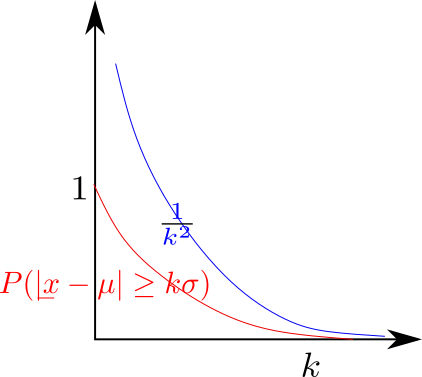
\includegraphics[width=2in]
{conventions/cheby.png}
\caption{
Pictorial representation of
Chebyshev's Inequality (CI).
Markov's Inequality (MI) has a similar
representation, but $k$ is proportional
to $\sqrt{a}$,
so the upper bound
for MI goes as $1/a$
instead of $1/k^2$.
}
\label{fig-cheby}
\end{figure}

See Fig.\ref{fig-cheby}
for a pictorial
representation of CI.
Note that the CI approximation
is always
a bad approximation for small $k$,
and might not
become good even  for large $k$.
For example, if the $\rvx$ distribution
is a box centered at $\mu$,
then $P(|\rvx-\mu|\geq k\s)=0$
for $k\s$ larger than the
width of the box,
so $1/k^2$
is a terrible approximation
for large $k$ too.

\hrule
A (1 dimensional) Center
of Mass (CM)
for a unit
mass object is an expectation
value where the
probability distribution
is a mass distribution.
Hence, it's not too surprising that
MI can be interpreted
in terms of CMs.

{\bf Physics Intuition for MI in terms of CMs:}

\beq
\underbrace{\int_0^{\infty}dx\; x P(x)
}_{E[\rvx]=CM}
=
\underbrace{
\frac{\int_0^a dx\; x P(x)}
{P(\rvx<a)}
}_{E_{\rvx<a}[\rvx]=CM^-}
\underbrace{P(\rvx<a)}_{f^-}
+
\underbrace{
\frac{\int_a ^{\infty}dx\; x P(x)}
{P(\rvx>a)}
}_{E_{\rvx>a}[\rvx]=CM^+}
\underbrace{P(\rvx>a)}_{f^+}
\eeq


\beqa
CM
\underbrace{(f^+ + f^-)}
_{=1}
&=&  CM^-f^- +  CM^+f^+
\\
&\geq&
 CM^+f^+
\\
&\geq&
a f^+
\quad \text{(because $CM^+\geq a$)}
\eeqa
You can think of $CM^+f^+$
as a torque with
moment arm= $CM^+$
and force=$f^+$.
In this picture,
MI is the approximation
of a torque with
moment arm=CM  and
force=1,
by a smaller torque with
moment arm= any real $a>0$
and force=$f^+\leq 1$.

\section{Short Summary of
Boolean Algebra}
See Ref.\cite{wiki-bool} for more info
about this topic.

Suppose $x, y, z\in \bool$. Define

\beq
x\text{ or }y=x\V y= x+y-xy
\;,
\eeq

\beq
x \text{ and }y=x\A y= xy
\;,
\eeq
and

\beq
\text{not }x=\ol{x}=1-x
\;,
\eeq
where we are using
normal addition and multiplication
on the right hand sides.\footnote{Note the
difference between $\V$ and modulus
2 addition $\oplus$.
For $\oplus$ (a.k.a. XOR): $x\oplus y=x+y-2xy$.}



\begin{table}[h!]
\centering
\begin{tabular}{|
>{\columncolor[HTML]{ECF4FF}}l |l|}
\hline
Associativity & \begin{tabular}[c]{@{}l@{}}$x \V (y \V z)=(x \V y) \V z$\\ $x \A (y \A z)=(x \A y) \A z$\end{tabular} \\ \hline
Commutativity & \begin{tabular}[c]{@{}l@{}}$x \V y=y \V x$\\ $x \A y=y \A x$\end{tabular} \\ \hline
Distributivity & \begin{tabular}[c]{@{}l@{}}$x \A (y \V z)=(x \A y) \V (x \A z)$\\ $x \V (y \A z)=(x \V y) \A (x \V z)$\end{tabular} \\ \hline
Identity & \begin{tabular}[c]{@{}l@{}}$x \V 0=x$\\ $x \A 1=x$\end{tabular} \\ \hline
Annihilator & \begin{tabular}[c]{@{}l@{}}$x \A 0=0$\\ $x \V 1= 1$\end{tabular} \\ \hline
Idempotence & \begin{tabular}[c]{@{}l@{}}$x \V x= x$\\ $x \A x= x$\end{tabular} \\ \hline
Absorption & \begin{tabular}[c]{@{}l@{}}$x \A (x \V y)= x$\\ $x \V (x \A y)= x$\end{tabular} \\ \hline
Complementation & \begin{tabular}[c]{@{}l@{}}$x \A \ol{x} = 0$\\ $x \V \ol{x}   = 1$\end{tabular} \\ \hline
Double negation & $\ol{(\ol{x})} = x$ \\ \hline
De Morgan Laws & \begin{tabular}[c]{@{}l@{}}$\ol{x} \A \ol{y} =\ol{(x \V y)}$\\ $\ol{x} \V \ol{y} = \ol{(x \A y)}$\end{tabular} \\ \hline
\end{tabular}
\caption{Boolean Algebra Identities}
\label{tab-bool-alg}
\end{table}

Actually, since
$x\A y=xy$, we can omit writing
the symbol $\A$. The symbol
$\A$ is useful to
exhibit the symmetry
of the identities, and
to remark
about
the analogous identities
for sets, where
$\A$ becomes intersection $\cap$
and $\V$ becomes union $\cup$. However,
for practical calculations,
$\A$ is an unnecessary nuisance.

Since $x\in \bool$,
\beq
P(\ol{x})=1-P(x)
\;.
\eeq

Clearly, from analyzing
the simple event space $(x,y)\in \bool^2$,
\beq
P(x\V y)= P(x) + P(y) - P(x\A y)
\;.
\eeq

\section{Laplace transform}
\label{sec-laplace-trans}

This section
is a watered down version
of the Wikipedia entry
for
Laplace Transforms
(Ref.\cite{wiki-laplace-transform}), which we highly recommend.

Let $0^- = 0-\eps$,
$0^+=0+\eps$
for some $\eps\in \RR$
such that $0<\eps<<1$.

Let $s=\s + i\omega$
for $\s,\omega\in\RR$.
$\s$ is called
the {\bf decay
constant}
and $\omega$
is called the
{\bf angular frequency}.

The {\bf Laplace Transform (LT)} of $f:[0,\infty]\rarrow \CC$
is defined as
\beq
\call[f](s)=\TIL{f}(s)=
\int_{0-}^\infty dt\; e^{-st} f(t)
\label{eq-def-lap-trans}
\eeq

Note that the LT is a linear functional\footnote{
A functional $\calf[f]$ is a function
of a function $f$,
or,
equivalently,
a function
of a vector
with possibly
infinitely
many components
given by $[f(x)]_{\forall x}$.}
because

\beq
\call[af+bg](t)
=
a\call[f](t)
+
b\call[g](t)
\eeq
for $f,g:[0, \infty]\rarrow \CC$
and $a,b\in\CC$.

The {\bf Inverse
Laplace Transform}
is defined so that

\beq \call^{-1}[\underbrace{\call[f]}_{\TIL{f}}](t)
= f(t)
\eeq

For LTs,
we assume functions
$f(t)$ that
vanish for $t<0^-$.
They can jump
to a finite value (with a step function) or
an infinite value
(with a Dirac delta function)
at $t=0$,
but must vanish for $t<0^-$.
LTs are ideally
suited for solving
ordinary
differential
equations
with {\bf initial conditions}
such as $x(0)=5$, $\partial_t x(0)=10$.




\begin{table}[h!]
\centering
\begin{tabular}{|l|l|l|}
\hline
\rowcolor[HTML]{ECF4FF}
name & formula & comment \\ \hline
\begin{tabular}{l}
 {\bf Bilateral Laplace}\\ {\bf transform (BLT)}
 \end{tabular}& $\calb[f](s)=\int_{-\infty}^\infty dt\; e^{-st} f(t)$ & \begin{tabular}[c]{@{}l@{}}same as LT but\\ with $-\infty<t<\infty$\\ instead of $t>0$\end{tabular} \\ \hline
{\bf Fourier transform (FT)} & $\calf[f](\omega)=\int_{-\infty}^\infty dt\; e^{-i\omega t} f(t)$ & \begin{tabular}[c]{@{}l@{}}Same as BLT but\\ with $s=i\omega\in i\RR$\end{tabular}
\\ \hline
{\bf Star Transform (ST)} & $\call^*[f](s)=\sum_{n=0}^\infty  e^{-snT} f(nT)$ & \begin{tabular}[c]{@{}l@{}}Same as LT but\\ it samples only\\ discrete points at
\\ $t=nT$\end{tabular} \\ \hline
\begin{tabular}{l}
{\bf Moment Generating}\\
{\bf Function}
\end{tabular}
&
\begin{tabular}{l}
$E_\rvx[e^{-s\rvx}]=\int_0^\infty
dx\;  e^{-sx} P(x)$\\
$\av{\rvx^n} = \left[(-\partial_\rvs)^n E_\rvx[e^{-s\rvx}]\right]_{s=0}$
\end{tabular}
 & \begin{tabular}[c]{@{}l@{}}Same as LT but\\
for probability \\ distribution
\\
$P:[0,\infty]\rarrow[0,1]$
\end{tabular} \\ \hline
\end{tabular}
\caption{Transforms that are akin to the Laplace transform.
Don't be intimidated by all these
transforms.
They are all
just
fancy
dot products
like $\vec{a}\cdot\vec{b}$.}
\label{tab-akin-to-LT}
\end{table}
Table
\ref{tab-akin-to-LT}
is a table of transforms
that are akin to the LT.
If the function $f(t)$
does not vanish for $t<0$,
we can use the
{\bf Bilateral Laplace Transform (BLT)}.
The BLT becomes the
{\bf Fourier transform (FT)} when
$s=i\omega$.
In this section,
we will only discuss the LT.

The following
intuition
about LTs might
be helpful to the reader.
A LT is like
a dot product of two vectors,
$e^{-st}$ and $f(t)$,
except that
in this case
the index $t$ for
their components
is an uncountable set $[0,\infty)$.
As with all
dot products, its maximum
is achieved
if the two vectors
point in the same
direction (this is
what the Cauchy Schwartz
inequality
$\vec{a}\cdot\vec{b}=
|\vec{a}||\vec{b}|\cos\theta
\leq |\vec{a}||\vec{b}|$
says).
In this case, if we substitute
$f(t) =\TIL{f}(s_0)e^{s_0t}$
on the right hand side
of Eq.(\ref{eq-def-lap-trans}),
we get

\beqa
\TIL{f}(s)
&=&
\TIL{f}(s_0)
\int_{0^-}^\infty
dt\; e^{-(s-s_0)t}
\\
&=&
\TIL{f}(s_0)\delta_+(s-s_0)
\eeqa
So our intuition
is this:
whenever you see
an equation
involving LTs,
replace each $f(t)$
by the special case
$f(t)= e^{s_ot}\TIL{f}$
(this is called a {\bf phasor}
when $s_0 = i\omega_0$),
and convince
yourself that
the equation
is valid
in the special case of phasors.



Define the {\bf Dirac delta function} by

\beq
\delta(t) =\int_{-\infty}^{\infty}
d\omega\; e^{i\omega t}
=
\left\{
\begin{array}{ll}
\infty & \text{if $t=0$}
\\
0 &\text{otherwise}
\end{array}
\right.
\eeq
and the
{\bf Heaviside step function} by

\beq
\heavy_a(t)=
\indi(t-a>0)
\eeq



Next, we
will list
some examples and
properties of
LTs.
Henceforth,
we will
use the following
notation:

$a, b\in\CC$

$f,g:[0,\infty]\rarrow \CC$

$f(t)\maparrow{\call} \TIL{f}(s)$ means
$\call[f](s) =\TIL{f}(s)$



\subsection{Examples}
\begin{itemize}

\item
Dirac delta function

\beq
\delta(t-a)
\maparrow{\call}
e^{-sa}
\eeq

\item
Heaviside step function



\beq
\heavy_a(t)
\maparrow{\call}
\frac{1}{s}
e^{-sa}\quad \text{(for $Re(s)>0$, $a>0$)}
\eeq

\item box

\beq
\heavy_0(t) - \heavy_a(t)
\maparrow{\call} \frac{1}{s}
(1-e^{-sa})\quad\text{(for $Re(s)>0$, $a>0$)}
\eeq

\item ramp

\beq
t\;\heavy_0(t)
\maparrow{\call}
\frac{1}{s^2}
\quad\text{(for $Re(s)>0$)}
\eeq

\item curved ramp

\beq
\frac{t^n}{n!}\heavy_0(t)
\maparrow{\call}
\frac{1}{s^{n+1}}
\quad \text{(for $Re(s)>0$ and $n\geq 0$)}
\eeq

\item sine, cosine

\beq
\sin(at)\heavy_0(t) \maparrow{\call}
\frac{a}{s^2+a^2}
\eeq

\beq
\cos(at)\heavy_0(t) \maparrow{\call}
\frac{s}{s^2+a^2}
\eeq

\item
polynomial rise, exponential drop

\beq
\frac{t^n}{n!}e^{-at}\;\heavy_0(t)
\maparrow{\call}
\frac{1}{(s+a)^{n+1}}
\quad\text{(for $Re(s)>-a$)}
\eeq

\item Exponential approach to steady state

\beq
(1-e^{-at})\heavy_0(t)
\maparrow{\call}
\frac{a}{s(s+a)}
\quad \text{(for $Re(s)>0, Re(s)>-a$)}
\eeq
\end{itemize}

\subsection{Properties}

\begin{itemize}

\item Taylor series of $f(t)$

\beq
\int_0^\infty
dx\;e^{ -x} \frac{x^n}{n!}
=1
\eeq

\beq
\int_0^\infty dt\;e^{-st} \frac{t^n}{n!}
=\frac{1}{s^{n+1}}
\eeq

\beq
\frac{t^n}{n!}\heavy_0(t)
\maparrow{\call}\frac{1}{s^{n+1}}
\eeq

\beqa
f(t)\heavy_0(t)&=&
\heavy_0(t)
\sum_{n=0}^\infty
\frac{t^n}
{n!}\partial_t^n f(0)
\\
&\maparrow{\call}&
\sum_{n=0}^\infty \frac{1}{s^{n+1}}
\partial_t^n f(0)
\eeqa

\item
derivatives of $\TIL{f}(s)$

\beq
(-t)f(t)
\maparrow{\call}
 \partial_s
\TIL{f}(s)
\eeq

\beq
(-t)^kf(t)
\maparrow{\call} (\partial_s)^k
\TIL{f}(s)
\eeq

\item
derivatives of $f(t)$

Define

\beq
f^{\geq 1}(t)
=f(t) -
f(0^+)\heavy_0(t)
\eeq


\beq
f^{\geq 2}(t)
= f(t) -
f(0^+)\heavy_0(t) - t f'(0^+)\heavy_0(t)
\eeq

\beqa
\partial_t f(t)
&\maparrow{\call}&
s
\TIL{f^{\geq 1}}(s)
\\
&=&
s\TIL{f}(s) - f(0^+)
\quad \text{(a.k.a. $f(t)$ {\bf differentiator})}
\label{eq-differentiator-lt}
\eeqa
For example, for $f(t)=\frac{t^n}{n!}\heavy_0(t)$,
we have $\TIL{f}(s)=\frac{1}{s^{n+1}}$,
so Eq.(\ref{eq-differentiator-lt}) becomes

\beq
\frac{t^{n-1}}{(n-1)!}
\maparrow{\call}
\frac{1}{s^{n}}
\eeq



\beqa
(\partial_t)^2 f(t)
&\maparrow{\call}&
s^2
\TIL{f^{\geq 2}}(s)
\\
&=&
s^2\TIL{f}(s)- sf'(0^+)- f(0^+)
\eeqa

\item
integral of $f(t)$ (a.k.a. $f(t)$
{\bf integrator})

\beq
\int_0^t d\tau\; f(\tau)
\maparrow{\call}
\frac{1}{s}\TIL{f}(s)
\label{eq-integrator-lt}
\eeq
For example,
for $f(t)=\frac{t^n}{n!}\heavy_0(t)$,
we have
$\TIL{f}(s)=\frac{1}{s^{n+1}}$,
so Eq.(\ref{eq-integrator-lt})
becomes

\beq
\frac{t^{n+1}}{(n+1)!}\heavy_0(t)
\maparrow{\call}
\frac{1}{s^{n+2}}
\eeq


Note that

\beqa
\int_0^t d\tau\; f(\tau)
&=&
\int_{-\infty}^\infty d\tau\; f(\tau)
\heavy_0(\tau)\heavy_0(t-\tau)
\\
&=&
((f \heavy_0)\circledast  \heavy_0)(t)
\eeqa


\item
integral of $\TIL{f}(s)$

\beq \frac{1}{t}f(t)
\maparrow{\call}
\int_s^\infty d\s\; \TIL{f}(\s)
\eeq

\item shifting $\TIL{f}(s)$ (frequency shifting)



\beq
e^{at}f(t)\maparrow{\call} \TIL{f}(s-a)
\quad\text{(for  $a>0$)}
\eeq



\item shifting $f(t)$ (time shifting).



\beq
f(t-a)\;\heavy_a(t)\maparrow{\call}
e^{-as}\TIL{f}(s)
\quad\text{(for  $a>0$)}
\eeq


\item time scaling

\beq
f(at)
\maparrow{\call}
\frac{1}{a}
\TIL{f}
\left(\frac{s}{a}\right)
\quad\text{(for  $a>0$)}
\eeq

\item multiplication

\beq
f(t)g(t)
\maparrow{\call}
\frac{1}{2\pi i}
\lim_{T\rarrow \infty}
\int_{c-iT}^{c+iT}
ds'\;
\TIL{f}(s')
\TIL{g}(s-s')
\eeq


\item convolution

The {\bf convolution}
of $f:\RR\rarrow\CC$
and $g:\RR\rarrow\CC$
is defined by
\beq
(f\circledast  g)(t) = \int_{-\infty}^\infty
d\tau\; f(\tau)g(t-\tau)
\eeq
If $f(t)=g(t)=0$
for $t<0$,

\beq
(f\circledast  g)(t) = \int_{0}^t
d\tau\; f(\tau)g(t-\tau)
\quad
\text{(see Fig.\ref{fig-convolution}.)}
\label{eq-conv-left-half-zero}
\eeq

\begin{figure}[h!]
\centering
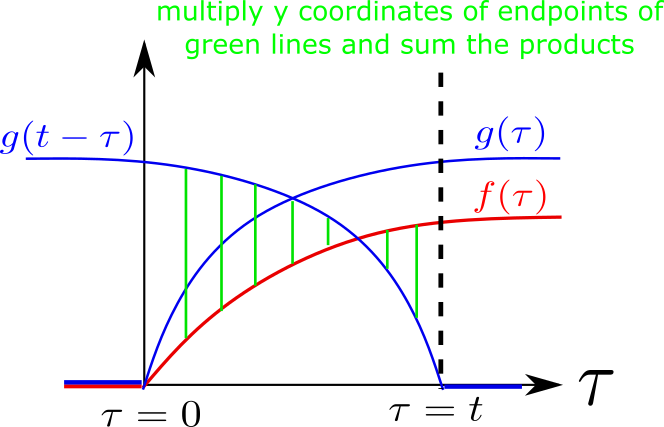
\includegraphics[width=3.5in]
{conventions/convolution.png}
\caption{Pictorial
representation
of the convolution
$(f\circledast g)(t)$. }
\label{fig-convolution}
\end{figure}

It's not hard to show that

\beq
f\circledast g = g\circledast f
\eeq
and that

\beq
(f\circledast  g)(t) \maparrow{\call}\TIL{f}(s)\TIL{g}(s)
\label{eq-lt-conv}
\eeq
Eq.(\ref{eq-lt-conv})
is easy to check
with phasors.
Indeed, if we substitute
$f(\tau)=e^{i\omega_0\tau}\TIL{f}$
and
$g(t-\tau)=
e^{i\omega_0(t-\tau)}\TIL{g}$,
on the right hand side
of Eq.(\ref{eq-conv-left-half-zero}),
the right
hand side
becomes $e^{i\omega_0t}\TIL{f}
\TIL{g}$,
and the LT of that
is $\TIL{f}
\TIL{g}$.

A common question
is how does one
evaluate
convolutions in practice.
If one can sample and remember
the waveforms $f(\tau)$
and $g(\tau)$
for all $\tau\in[0,t]$,
then it's just a matter
of multiplication
and addition of samples.
Sometimes, even if we
have no memory resources,
it's possible to calculate a convolution. For example,
if $g(t)=e^{st}\heavy_0(t)$

\beqa
(f\circledast g)(t)
&=&
\int_0^t d\tau\;
f(\tau)e^{s(t-\tau)}
\\
&=&
\underbrace{e^{st}}_
{g(t)}\TIL{f}(s)
\eeqa
so convolving this $g(\cdot)$
merely evaluates it at $t$
and multiplies it
by a constant $\TIL{f}(s)$.

\item circular convolution

If $f_T, g_T$ are
periodic functions
with period $T$,
their
{\bf circular convolution}
is defined as

\beq
(f_T\circledast_C g_T)(t)
=
\int_0^Td\tau\;
f_T(\tau)g_T(t-\tau)
\eeq
One can show that

\beq
(f_T\circledast_C g_T)(t)
\maparrow{\call}
\TIL{f_T}(s) \TIL{g_T}(s)
\eeq

\item complex
conjugation
\beq
f^*(t)\maparrow{\call}\TIL{f}^*(s^*)
\eeq

\item cross correlation

The {\bf cross correlation}
of functions $f,g:[0, \infty]\rarrow\CC$
is defined as

\beq
(f,g)_{CC}=
\int_0^\infty
d\tau\;
f^*(\tau)
g(t+\tau)
\eeq
One can show that

\beq
(f,g)_{CC}
\maparrow{\call}
\TIL{f}^*(-s^*)\TIL{g}(s)
\eeq

\item LT of periodic function

If $f_T(t)$ is a periodic function
with period $T$, then

\beq
f_T(t) \heavy_0(t)\maparrow{\call}
\frac{1}{1-e^{-sT}}
\int_0^T dt\;
e^{-st}f_T(t)
\eeq

To show this, define
\beq
\cali_a^b=
\int_a^b dt\;
e^{-st}f_T(t)
\eeq
Then

\beqa
\TIL{f_T}(s)
&=& \cali_0^T + \cali_{T}^{2T}
+
\cali_{2T}^{3T}+\cdots
\\
&=&
\cali_0^T(1 + e^{-sT} + e^{-s2T} +\cdots)
\\
&=&
\frac{1}{1-e^{-sT}}\cali_0^T
\eeqa



\item
periodic summation

\beq
\sum_{n=0}^\infty
f(t-nT)\heavy_0(t-nT)
\maparrow{\call}
\frac{1}{1{\color{red}-}e^{-Ts}}
\TIL{f}(s)
\eeq

\beq
\sum_{n=0}^\infty
{\color{red}(-1)^n}
f(t-nT)\heavy_0(t-nT)
\maparrow{\call}
\frac{1}{1{\color{red}+}e^{-Ts}}
\TIL{f}(s)
\eeq

\item limits of $f(t)$


\beqa
\lim_{s\rarrow \infty}s\TIL{f}(s)
&=&
\lim_{s\rarrow \infty}s\int_0^\infty dt\; e^{-st}f(t)
\\
&\approx&
f(0^+)\lim_{s\rarrow \infty}
\underbrace{s\int_0^\infty dt\; e^{-st}
}_{=1}
\\
&=&
f(0^+)
\eeqa

\beq
\lim_{s\rarrow 0}s\TIL{f}(s)
= f(\infty) \quad\text{(a.k.a. steady state)}
\eeq

\item Inverse LT

The inverse
LT of a function
$\TIL{f}(s)$
can be calculated
by performing
the
following
complex contour integral:

\beq
\underbrace{\call^{-1}[\TIL{f}(s)](t)}_
{f(t)} = \frac{1}{2\pi i}
\lim_{T\rarrow \infty}
\int_{\gamma-iT}^{\gamma+iT}ds\;
e^{st}\TIL{f}(s)
\eeq
where $\gamma, T\in\RR$
and all singularities
of $\TIL{f}(s)$ must
be located on the left side of the contour of integration.
Another way of calculating
the inverse LT of $\TIL{f}(s)$, is
to express
$\TIL{f}(s)$ as a linear combination
of functions for which the inverse LT
is known from LT tables. For instance,

\begin{align}
\call^{-1}
\left[
\frac{1}{s(s-1)}
\right]
=&
\call^{-1}
\left[
\frac{1}{s} - \frac{1}{s+1}
\right] \text{(partial fractions expansion)}
\\
=&
\call^{-1}
\left[
\frac{1}{s}\right]
 - \call^{-1}
 \left[\frac{1}{s+1}\right]
 \\
 =&
 \heavy_0(t)[1-e^{-t}]
\end{align}

\item {Bode, Nyquist plots}

Let $s=\s+i\omega$.

{\bf Bode plot}: plot of
$$(\log_{10}(\omega),
\log_{10}|\TIL{f}(i\omega)|)$$ and,
right below it, plot of
$$(\log_{10}(\omega),
phase\{\TIL{f}(i\omega)\})$$.

{\bf Nyquist plot}: plot of
$$(Re \TIL{f}(i\omega), Im \TIL{f}(i\omega))$$
or, equivalently,
plot of

$$(|\TIL{f}(i\omega)|, phase(\TIL{f}(i\omega)))$$
on polar graph paper.

Usually, $\TIL{f}(i\omega)$
is a gain (i.e.,  LT
of output
divided by LT
of input).

\item uncertainty principle

Here is some
\qt{Heisenberg uncertainty
principle} type intuition
about the relationship
between a function
$f(t)$ and its LT $\TIL{f}(s)$
for $s=i\omega\in i\RR$.

\beq
\begin{array}{c|c|c|c}
f(t)&\TIL{f}(i\omega)
&|\TIL{f}(i\omega)|&
phase(\TIL{f}(i\omega))
\\ \hline\hline
\delta(t)
&1
&1
&0
\\
\heavy_0(t)
&
\frac{1}
{i\omega}
&\frac{1}{|\omega|}
&-\frac{\pi}{2}
\\
t\;\heavy_0(t)
&
\frac{1}
{(i\omega)^2}
&
\frac{1}{\omega^2}
&
-\pi
\\
\frac{t^2}{2} \heavy_0(t)
&
\frac{1}
{(i\omega)^3 }
&
\frac{1}{|\omega|^3}
&
\frac{\pi}{2}
\end{array}
\eeq
Hence, the narrower $f(t)$ is,
the broader $|\TIL{f}(i\omega)|$ is.
Also, the more
$f(t)$ is a high pass filter,
the more
$|\TIL{f}(i\omega)|$
is a low pass filter.



\end{itemize}

\section{Z-transform}
\label{sec-z-transform}

This section
is a watered down version
of the Wikipedia entry
for
Z-transforms
(Ref.\cite{wiki-z-transform}), which we highly recommend.
Before reading
this section,
we recommend that the
reader read Section \ref{sec-laplace-trans}
on Laplace transforms,
as those are the continuous
in time version of Z-transforms.

Suppose $x^{[n]}\in\CC$
for all $n\in \ZZ^{\geq 0}$ ($\ZZ^{\geq 0}=$non-negative
integers), and $z\in \CC$. Then
we define the {\bf Z-transform (ZT)} by
\beq
\calz{[x]}(z)=
\TIL{x}(z) =
\sum_{n=0}^\infty x^{[n]} z^{-n}
\eeq

Note that the ZT is a linear functional
because

\beq
\calz[a x^{[n]} + b y^{[n]}]=
a\calz[x^{[n]}]
+
b\calz[y^{[n]}]
\eeq
for $x^{[n]}, y^{[n]}\in\CC$
for all $n\in \ZZ^{\geq 0}$, and $a,b\in\CC$.

The {\bf Inverse
Z-transform}
is defined so that

\beq \calz^{-1}[\underbrace{\calz[x^{[n]}]}
_{\TIL{x}(z)}]^{[n]}
= x^{[n]}
\eeq

\begin{table}[h!]
\centering
\begin{tabular}{|l|l|l|}
\hline
\rowcolor[HTML]{ECF4FF}
name & formula & comment \\ \hline
\begin{tabular}{l}
{\bf Bilateral}
\\{\bf ZT (BZT)}
\end{tabular} & $\TIL{x}(z)=\sum_{n=-\infty}^\infty x^{[n]} z^{-n}$ & \begin{tabular}[c]{@{}l@{}}Same as ZT but\\ with $n\in \ZZ$\\ instead of \\ $n\in\ZZ^{\geq 0}$\end{tabular} \\ \hline
\begin{tabular}{l}
{\bf Discrete time Fourier}\\
{\bf transform (DTFT)}
\end{tabular} & $\TIL{x}_{2\pi}(\omega)=\sum_{n=-\infty}^{\infty}x^{[n]}e^{-i\omega n}$ & \begin{tabular}[c]{@{}l@{}}same as BZT but \\ with $z = e^{i\omega}$\end{tabular} \\ \hline
\begin{tabular}{l}
{\bf Discrete Fourier}
\\
{\bf transform (DFT)}
\end{tabular} & $\TIL{x}^{[k]}=\sum_{n=0}^{N-1}x^{[n]} e^{-i \frac{2\pi kn}{N}}$ & \begin{tabular}[c]{@{}l@{}}Same as  ZT but a\\finite ($N$) number of\\ $x^{[n]}$ components, and\\ with $z=e^{i\frac{2\pi k}{N}}$ for
\\
$k=0, 1, \dots, N-1$
\\
(N roots of unity\\
on unit circle)\end{tabular} \\ \hline
\begin{tabular}{l}
{\bf Probability}\\
{\bf Generating Function}
\end{tabular} & $\TIL{P}(z)=\sum_{n=0}^{\infty}P^{[n]}
z^n$ & \begin{tabular}[c]{@{}l@{}}same as ZT but \\ with $n\rarrow -n$
and \\
$P^{[n]}:\ZZ^{\geq 0} \rarrow [0,1]$
\\
is a discrete prob.
\\
distribution. If \\
$z=e^{-T}$, get moment\\
genetating function.
\end{tabular} \\
\hline
\end{tabular}
\caption{Transforms that are akin to the Z-transform.
Don't be intimidated by all these
transforms.
They are all
just
fancy
dot products
like $\vec{a}\cdot\vec{b}$.}
\label{tab-akin-to-ZT}
\end{table}
Table \ref{tab-akin-to-ZT}
is a table of
transforms that are akin to
the ZT.

For models that are
continuous in time (i.e., analog)
we use Laplace transforms (LTs),
and for models that are discrete in time
(i.e., digital),
we use Z-transforms (ZTs).
Digital models
are often obtained
by sampling analog models
at discrete times separated by
a time interval $T$.
Hence, it is useful
to know how LTs and ZTs
are related. To find out, let

\beq
e^{-st}=z^{-n}
\eeq
and

\beq
t=nT
\eeq
Hence, we arrive at the
very useful formula

\beq
\boxed{
z= e^{sT}}
\eeq
\begin{figure}[h!]
\centering
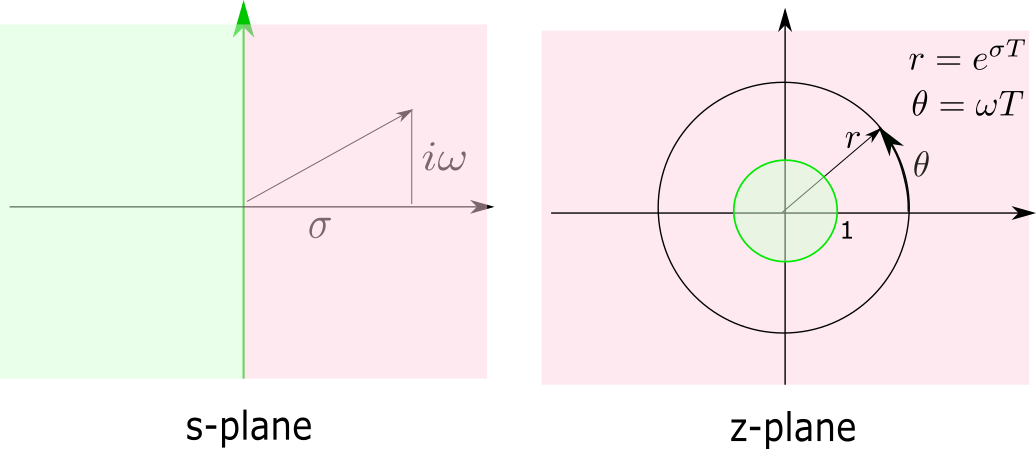
\includegraphics[width=5in]
{conventions/s-z-planes.png}
\caption{Relationship
between the s-plane (for Laplace transform)
and z-plane (for Z-transform.).}
\label{fig-s-z-planes}
\end{figure}

If

\beq
s=\s +i\omega, \quad
z = re^{i\theta}
\eeq
then

\beq
r =e^{\s T}
,\quad
\theta =\omega T
\label{eq-s-z-plane-map}
\eeq
The map given
by Eqs.(\ref{eq-s-z-plane-map})
is illustrated by Fig.\ref{fig-s-z-planes}.
As shown in Fig.\ref{fig-s-z-planes},
the map
from the s-plane (for
LTs)
to the z-plane (for ZTs) maps:

\begin{itemize}
\item
left half plane (LHP) $\rarrow$
inside of the unit
circle

\item
imaginary axis $\rarrow$ unit circle.
In particular, the s-plane origin $s=0$
and points with $\s=0, \omega=\frac{2\pi k}{T}$,
where $k\in\ZZ$,
are all mapped to $z=1$.

\item
right half plane (RHP) $\rarrow$ outside
of unit circle


\end{itemize}



Define the
{\bf Kronecker delta function} by

\beq
\delta_j^{[n]} = \indi(n=j)
\eeq
and the {\bf discrete Heavyside step
function} by

\beq
\heavy_j^{[n]}=\indi(n\geq j)
\eeq
Note that

\beq
H_0^{[n]}=\sum_{k=0}^\infty\delta^{[n]}_k
\eeq

Next, we
will list
some examples and
properties of
ZTs.
Henceforth,
we will
use the following
notation:

$x^{[n]}, x_1^{[n]}, x_2^{[n]}\in \CC$
are defined only for $n\in \ZZ^{\geq 0}$

$x^{[n]}\maparrow{\calz} \TIL{x}(z)$ means
$\calz[x^{[n]}] =\TIL{x}(z)$

The {\bf Region Of
Convergence (ROC)}
for a ZTs is very important
(Without knowing the ROC, you can't invert
a ZT $\TIL{x}(z)$). We won't list ROCs
 here, but they
can be found in ZT
tables like those in Ref.\cite{wiki-z-transform}.

\begin{mdframed}[hidealllines=true,backgroundcolor=blue!10]
Note that ZT  formulae
can be \qt{sanity checked} by
replacing
$z=e^{sT}$
and checking that
for $0<T<<1$,
\beq
 \calz[x](e^{sT})\approx
 \frac{1}{T}
\call[f](s)
\eeq

Note also that
for $T<<1$:

\beq
z\approx 1,\quad
z\partial_z=\partial_{
\ln z} =\partial_{sT},\quad
(z-1)^n\approx (sT)^n
\eeq

$\int_{0-}^\infty dt\; \delta(t)=1=
\sum_{n=0}^\infty\delta^{[n]}_0$ so
by dimensional
analysis, $\delta^{[n]}_0\approx T\delta(t)$.

$\heavy_0^{[n]}\approx \heavy_0(t)$

\end{mdframed}


\subsection{Examples}
\begin{itemize}

\item Kronecker delta function

\beq
\delta_{n_0}^{[n]}
\maparrow{\calz}
z^{-n_0}
\eeq

Compare this with

\beq
\delta(t-t_0)
\maparrow{\call} e^{-st_0}
\eeq
with $t_0=n_0T$
and $z=e^{sT}$.

Note that

\beqa
\calz[\heavy^{[n]}_0]
&=&
\sum_{k=0}^\infty\calz[\delta^{[n]}_k]
\\
&=&
\sum_{k=0}^\infty z^{-k}
\\
&=&
\frac{1}{1-1/z}
\eeqa


\item unit step

For $a\in\CC$,

\beq
a^n \heavy_0^{[n]}
\maparrow{\calz}
\frac{1}{1-az^{-1}}
\quad \text{for $|z|>|a|$}
\eeq


\beq
-a^n \heavy_0^{[-n-1]}
\maparrow{\calz}
\frac{1}{1-az^{-1}}
\quad \text{for $|z|<|a|$}
\eeq

Compare this with

\beq
\heavy_0(t)
\maparrow{\call}
\frac{1}{s}
\quad \text{\text{(for $Re(s)>0$)}}
\eeq
for $a=1$, $z=e^{sT}\approx 1 + sT$.


\item ramp

For $a\in\CC$,

\beq
n a^n \heavy_0^{[n]}
\maparrow{\calz}
\frac{az^{-1}}{(1-az^{-1})^2}
\quad \text{for $|z|>|a|$}
\eeq


\beq
-n a^n \heavy_0^{[-n-1]}
\maparrow{\calz}
\frac{az^{-1}}{(1-az^{-1})^2}
\quad \text{for $|z|<|a|$}
\eeq

\item sine, cosine

For $a\in\CC$,

\beq
a^n\sin(\omega_0n)\heavy_0^{[n]}
\maparrow{\calz}
\frac{az^{-1}\sin\omega_0}
{1-2az^{-1}\cos\omega_0 + a^2 z^{-2}}
\eeq

\beq
a^n\cos(\omega_0n)\heavy_0^{[n]}
\maparrow{\calz}
\frac{1-az^{-1}\cos\omega_0}
{1-2az^{-1}\cos\omega_0 + a^2 z^{-2}}
\eeq
\end{itemize}

\subsection{Properties}
\begin{itemize}
\item time expansion

\beq
x^{[n/K]}\indi(n/K\in\ZZ)
\maparrow{\calz}
\TIL{x}(z^K)
\eeq

\item decimation
\beq
x^{[Kn]}
\maparrow{\calz}
\frac{1}{K}
\sum_{p=0}^{K-1}
\TIL{x}\left(
z^{\frac{1}{K}}
e^{-i 2\pi \frac{p}{K}}
\right)
\eeq

\item time delay

\beq
x^{[n-k]}
\maparrow{\calz}
z^{-k}\TIL{x}(z)
\quad \text{(for $k>0$)}
\eeq

\item time advance

\beq
x^{[n+k]}
\maparrow{\calz}
z^{k}
\left(
\TIL{x}(z)
-z^k\sum_{n=0}^{k-1}
x^{[n]}z^{-n}
\right)
\quad \text{(for $k>0$)}
\eeq

\item first difference backwards

\beq
x^{[n]}
-x^{[n-1]}
\maparrow{\calz}
(1-z^{-1})\TIL{x}(z)
\eeq

\item first difference forward

\beq
x^{[n+1]}
-x^{[n]}
\maparrow{\calz}
z\left( (1-z^{-1})
\TIL{x} -x^{[0]}
\right)
\eeq

\item time reversal

\beq
x^{[-n]}
\maparrow{\calz}
\TIL{x}(z^{-1})
\eeq

\item scaling in z-domain

For $a\in\CC$,

\beq
a^n x^{[n]}
\maparrow{\calz}
\TIL{x}(a^{-1}z)
\eeq

\item complex conjugation

\beq
(x^{[n]})^*
\maparrow{\calz} \TIL{x}^*(z^*)
\eeq

\beq
Re(x^{[n]})
\maparrow{\calz}
\frac{1}{2}
(\TIL{x}(z)+\TIL{x}^*(z^*))
\eeq

\beq
Im(x^{[n]})
\maparrow{\calz}
\frac{1}{2i}
(\TIL{x}(z)-\TIL{x}^*(z^*))
\eeq

\item $\TIL{x}(z)$ differentiation

\beq
nx^{[n]}
\maparrow{\calz}
-z\partial_z \TIL{x}(z)
\eeq

\item convolution

Define the {\bf (discrete)
convolution}
of $x_1^{[n]}$
and $x_2^{[n]}$ by

\beq
x_1^{[n]}\circledast x_2^{[n]}=
\sum_{k=0}^nx_1^{[k]}x_2^{[n-k]}
\eeq
One can show that

\beq
x_1^{[n]}\circledast x_2^{[n]}
\maparrow{\calz}
\TIL{x}_1(z)\TIL{x}_2(z)
\eeq

\item cross-correlation

\beq
(x_1^{[-n]})^*\circledast x_2^{[n]}
\maparrow{\calz}
\TIL{x_1}^*\left(\frac{1}{z^*}\right))
\TIL{x}_2(z)
\eeq

\item accumulation

\beq
\sum_{k=-\infty}^\infty
x^{[k]}
\maparrow{\calz}
\frac{1}{1-z^{-1}}
\TIL{x}(z)
\eeq

\item multiplication

\beq
x_1^{[n]} x_2^{[n]}
\maparrow{\calz}
\frac{1}{2\pi i}
\oint_C \frac{dw}{w}\;
\TIL{x}_1(w)
\TIL{x}_2\left(
{\color{red}\frac{z}{w}}
\right)
\eeq

\item Parseval's theorem

\beq
\sum_{k=-\infty}^{\infty}
x_1^{[n]}(x_2^{[n]})^*
=
\frac{1}{2\pi i}
\oint_C \frac{dw}{w}\;
\TIL{x}_1(w)
\TIL{x}_2^*\left(
{\color{red}
\frac{1}{w^*}}
\right)
\eeq

\item limits of $x^{[n]}$

initial value theorem

\beq
x^{[0]}=\lim_{z\rarrow \infty}
\TIL{x}(z)
\eeq

final value theorem

\beq
x^{[\infty]}=\lim_{z\rarrow 1}
(z-1)\TIL{x}(z)
\eeq

\item Inverse ZT

\beq
\underbrace{\calz^{-1}[\TIL{x}(z)]}
_{x^{[n]}}=
\frac{1}{2\pi i}
\oint_C dz\;
\TIL{x}(z)z^{n-1}
\eeq
where $C$
is a counterclockwise
closed path
containing the origin and
all singularities
of $\TIL{x}(z)$.

\end{itemize}


\section{Legendre Transformation (dual functions)}
\label{sec-dual-fun}
This section is a
watered down version of
the Wikipedia article
Ref.\cite{wiki-legendre-transformation},
which we highly recommend.



\begin{figure}[h!]
\centering
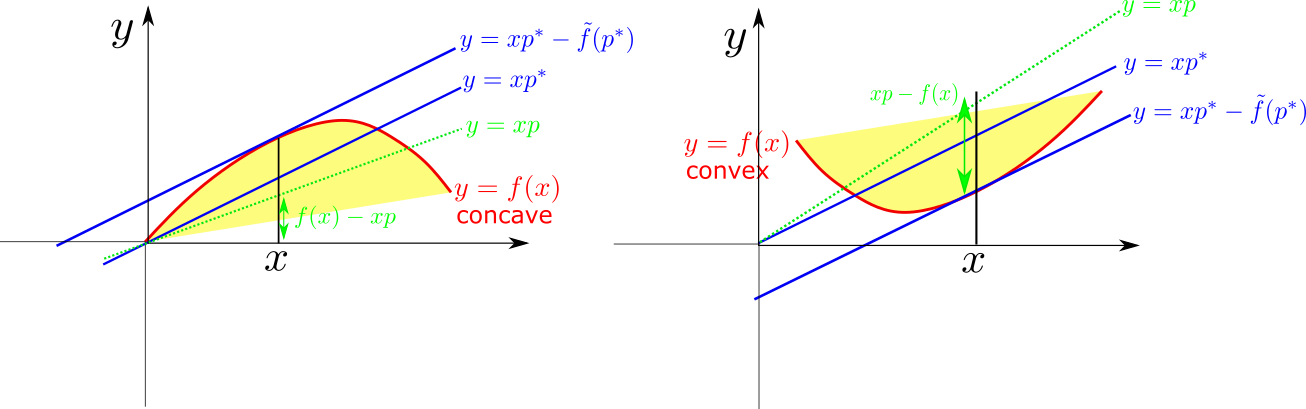
\includegraphics[width=6in]
{conventions/dual-fun-detail.png}
\caption{The line
$y=xp$ goes through the
origin and has arbitrary slope
$p$. $p^*$ is
the special slope
at $x$
for which the line
$y=xp^*$,
if
displaced parallelly,
can be made tangential (kissing)
to
the curve $y=f(x)$.}
\label{fig-dual-fun-detail}
\end{figure}

\begin{figure}[h!]
\centering
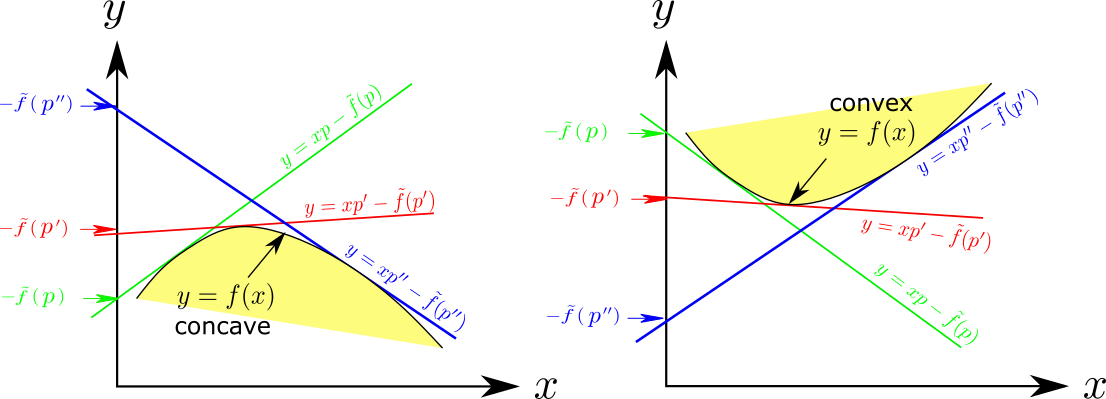
\includegraphics[width=6in]
{conventions/dual-fun.png}
\caption{The dual
function $\TIL{f}(p)$ of a concave or convex function
$f(x)$
is the osculating (kissing)
locus of the
family
of lines $y=px - \TIL{f}(p)$,
where $p$
is the slope at $x$
of the curve $y=f(x)$.}
\label{fig-dual-fun}
\end{figure}

Let $x,p\in\RR^n$.
If $f:\RR^n\rarrow \RR$ is a concave function, we
define its {\bf dual (a.k.a.
conjugate) function}
$\TIL{f}:\RR^n\rarrow \RR$ by

\beq
\TIL{f}(p) = \min_x (p^T x - f(x))
\label{eq-Fp-def}
\;.
\eeq
This definition also applies if
one replaces the words \qt{concave}
by \qt{convex} and
\qt{min} by \qt{max}.\footnote{This
book does not try to be
mathematically rigorous
beyond the level
of applied math. To be truly
rigorous and general,
replace \qt{max} by \qt{supremum}
and \qt{min} by \qt{infimum}.
Pure mathematicians use
min and max
only over finite sets,
but physicists and engineers
often discretize to obtain
a max or min  over a finite
set with $N$ points,
and then, afterwards,
take the limit $N\rarrow\infty$.
Not perfect, but good enough
for most applied work. }
$\TIL{f}(p)$
is also called the
{\bf Legendre transformation (or
Legendre transform)} (LT)
of $f(x)$.

In Physics, $x$ is the position
vector and $p$ is the momentum
vector of a system.

See Figs.
\ref{fig-dual-fun-detail}
and \ref{fig-dual-fun}
for a pictorial
representation
of LT.

Note that
the right hand side of
Eq.(\ref{eq-Fp-def})
implies that

\beq
\sum_i
(p_i-\partial_{x_i}
f(x))\delta x_i=0
\eeq
for all variations $\delta x_i$.
If minimization is achieved
when $x=x^*$, then

\beq
p= \nabla_{x^*} f(x^*),
\quad x^*=
(\nabla_{x^*} f)^{-1}(p)
\eeq

\subsection{Examples}

\begin{enumerate}
\item
Find the dual function of
\beq
\boxed{f(x) = e^x}
\;.
\eeq

\beqa
p &=& \partial_{x^*}f
\\
&=&
e^{x^*}
\eeqa

\beq
x^* = \ln  p
\eeq

\beq
f(x^*) = p
\eeq

\beqa
\TIL{f}(p)&=&x^*p - f(x^*)
\\
&=&
p\ln p -p
\eeqa



\hrule
\item
Find the dual function of
\beq
\boxed{f(x) = f + f'x +\frac{1}{2}f''x^2}
\;.
\eeq

\beqa
p&=&
\partial_{x^*} f
\\
&=&
f' + f''x^*
\label{eq-p-xstar}
\eeqa

\beq
x^* = \frac{p-f'}{f''}
\eeq
\beqa
f(x^*)&=& f
+
f'
\left[
\frac{p-f'}{f''}\right]
+
\frac{1}{2}f''
\left[\frac{p-f'}{f''}\right]^2
\\
&=&
\left[f - \frac{(f')^2}{2f''}\right]
+
p^2\left[
\frac{1}{2f''}
\right]
\eeqa

\beqa
\TIL{f}(p)&=&
px^*-f(x^*)
\\
&=&
p\left[\frac{p-f'}{f''}\right]
-f(x^*)
\\
&=&
\left[-f + \frac{(f')^2}{2f''}\right]
+
p\left[
\frac{-f'}{f''}
\right]
+
p^2\left[
\frac{1}{2f''}
\right]
\eeqa

Note that when $f=f'=0$,
we get

\beq
f(x)=\frac{f'' x^2}{2}
,\quad
\TIL{f}(p)= \frac{p^2}{2 f'' }
\eeq

Note that if $f$ is convex
(resp., concave), $\TIL{f}$
is convex too (resp., concave too).

%\beqa
%x &=&
%\partial_{p^*} \TIL{f}
%\\
%&=&
%\left[
%\frac{-f'}{f''}
%\right]
%+
%p^*\left[
%\frac{1}{f''}
%\right]
%\eeqa
%
%\beq
%p^* = f' + f''x
%\quad\text{(see Eq.(\ref{eq-p-xstar}))}
%\eeq
%
%\beqa
%\TIL{f}(p^*)&=&
%\left[-f + \frac{(f')^2}{2f''}\right]
%+
%[f' + xf'']
%\left[
%\frac{-f'}{f''}
%\right]
%+
%[f'+f''x]^2
%\left[
%\frac{1}{2f''}
%\right]
%\\
%&=&
%-f + \frac{f''}{2} x^2
%\eeqa
%
%
%\beqa
%f(x)&=& p^*x - \TIL{f}(p^*)
%\\
%&=&
%[f'+f'' x]x
%+f-\frac{f''}{2} x^2
%\\
%&=&
%f + f'x+\frac{f''}{2} x^2
%\eeqa

\hrule

\item
Find the dual function of
\beq
\boxed{f(x)= \ln(1-e^{-x})}
\;.
\eeq

\beqa
p
&=&
\partial_{x^*} f(x^*)
\\
&=&
\frac{e^{-x^*}}{1-e^{-x^*}}
\eeqa

\beq
p=(1+p)e^{-x^*}
\eeq
\beq
x^* = \ln\frac{1+p}{p}
\eeq

\beq
f(x^*)=\ln\left(
1 - \frac{p}{1+p}
\right)=-\ln(1+p)
\eeq

\beqa
\TIL{f}(p) &=& p x^* -f(x^*)
\\
&=&
p \ln\frac{1+p}{p}
+\ln(1+p)
\\
&=&
-p\ln  p
+(1+p)\ln(1+p)
\eeqa
\end{enumerate}


\begin{figure}[h!]
\centering
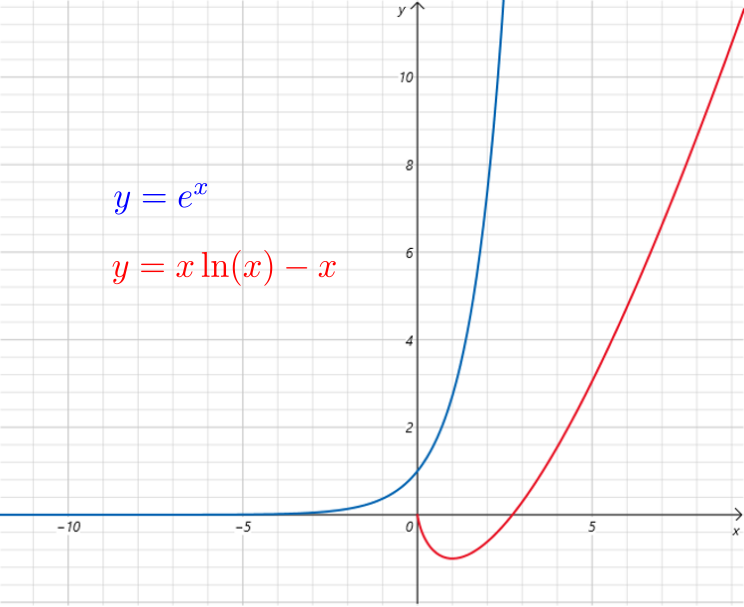
\includegraphics[width=3.5in]
{conventions/dual-ex.png}
\caption{$f(x)=e^x$ and its dual.}
\label{fig-dual-ex}
\end{figure}

\begin{figure}[h!]
\centering
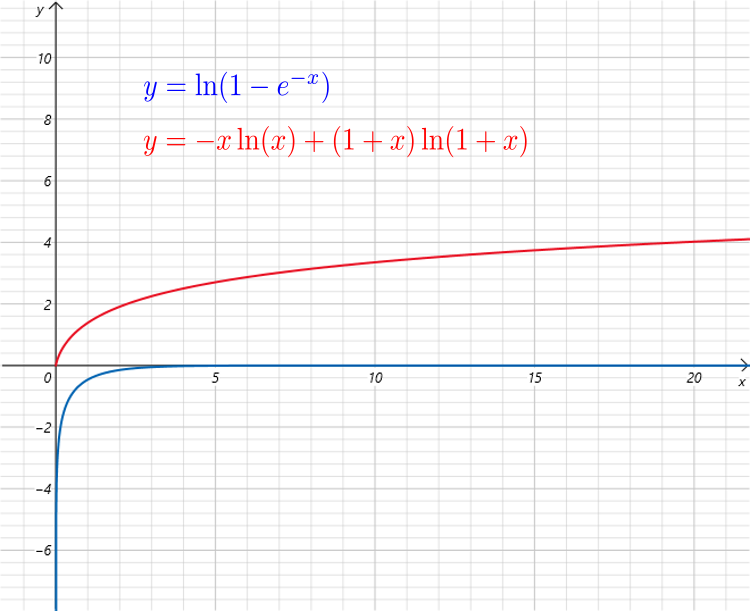
\includegraphics[width=3.5in]
{conventions/dual-ln-1-e-x.png}
\caption{$f(x)=\ln(1-e^{-x})$ and its dual.}
\label{fig-dual-dual-ln-1-e-x}
\end{figure}




\subsection{Properties}

\begin{claim}
If $f(x)$ is a concave function
with dual $\TIL{f}(p)$, then
\beq
f(x)= \min_p(p^T x - \TIL{f}(p))
\label{eq-fx-as-min}
\eeq

 \beq
 \nabla_p \TIL{f}(p(x)) = (\nabla_x f)^{-1}(x)
 \eeq
Eqs.(\ref{eq-Fp-def})
and (\ref{eq-fx-as-min})
are also true if we replace the
words \qt{concave} with \qt{convex}
and \qt{min} with \qt{max}.
\end{claim}
\proof

Let $x^*$
be the value of $x$
which minimizes $y=p^T x-f(x)$
with respect to $x$. Hence,
\beq
\TIL{f}(p) = p^Tx^* - f(x^*)
\;.
\label{eq-Fp}
\eeq
Rearranging terms in Eq.(\ref{eq-Fp}),
we get

\beq
f(x^*) = p^Tx^* - \TIL{f}(p)
\label{eq-relabel-1}
\eeq

Let $p^*$
be the value of $p$
which minimizes $y=p^T x-\TIL{f}(p)$
with respect to $p$. Hence,
\beq
f(x) = (p^*)^Tx - \TIL{f}(p^*)
\label{eq-relabel-2}
\eeq
Replacing $p^*$ by $p$
and $x$ by $x^*$
in Eq.(\ref{eq-relabel-2})
yield Eq.(\ref{eq-relabel-1}).


Note that minimization
with respect to $x$
is achieved if
\beq
p_i = \partial_{x_i}f(x),\;
p = \nabla_x f(x)
\eeq
whereas minimization
with respect to $p$
is achieved if

\beq
x_i = \partial_{p_i}\TIL{f}(p),\;x = \nabla_p \TIL{f}(p)
\eeq
Hence,

\beq
x = \nabla_p \TIL{f}(\nabla_x f(x))
\eeq

\qed

\begin{claim}
If $f(x)$ is concave
(resp., convex),
then $\TIL{f}(p)$
is also concave (resp., convex)
\end{claim}
\proof

\beq
\TIL{f}(p)
=
x^*p - f(x^*)
\eeq

\beq
\frac{d\TIL{f}}{dp}
=
x^* +
\underbrace{(p- f'(x^*))}_{=0}
\frac{dx^*}{dp}
= x^*
\eeq

\beq
\frac{d^2\TIL{f}}{dp^2}
=
\frac{dx^*}
{dp}
\eeq


\beq
p= f'(x^*),
\quad x^* = (f')^{-1}(p)
\eeq

\beq
dp = f''(x^*)dx^*,
\quad
\frac{dx^*}{dp}=
\frac{1}{f''(x^*)}
\eeq

\beq
\frac{d^2\TIL{f}}{dp^2}
=
\frac{1}{f''(x^*)}
\eeq



\qed

\begin{claim}
 LT is its own
 inverse (i.e., LT is
 a self-inverse
 or involution
 transformation)
\beq
\TIL{\TIL{f}}(x) = f(x)
\eeq
\end{claim}
\proof
$x=x_1, p=x_2$

\beq
\TIL{f}(x_2)=
x_2 x_1^* -f(x_1^*),
\quad
x_2=f'(x_1^*)
\eeq

\beq
\TIL{\TIL{f}}(x_3)=
x_3 x_2^* -\TIL{f}(x_2^*),
\quad
x_3=(\TIL{f})'(x_2^*)
\eeq

\beqa
\TIL{\TIL{f}}(x_3)&=&
x_3
x_2^*
-x_2^*
 x_1^* +f(x_1^*)
 \\
&=&
f(x_1^*) \quad \text{( for $x_1^*=x_3$)}
\eeqa

\beq
x=x_3=
(\TIL{f})'(x_2^*)=
(\TIL{f})'(f'(x_1^*))=x_1^*
\eeq





\qed

Additional properties
\begin{itemize}
\item Scaling
\beq
ag(bx)\maparrow{LT} a \TIL{g}(\frac{p}{ab})
\eeq
for $a,b>0$
\item Translation

\beq
g(x+y)+b
\maparrow{LT} \TIL{g}(p)-p^Ty -b
\eeq
\item Frenchel's inequality

\beq
p^Tx \leq f(x) + \TIL{f}(p)
\eeq

\end{itemize}



\subsection{Connection to Fourier transform
and Quantum Mechanics}

Recall how Fourier transforms (FTs)
arise in Quantum Mechanics.
Suppose $x,p\in\RR$ and
\beq
\psi(x)
=\av{x|\psi},
\quad
\TIL{\psi}(p)
=\av{p|\psi}
,\quad
\av{p|x}=
\frac{e^{-ipx}}{\sqrt{2\pi}}
\eeq
Then

\beqa
\TIL{\psi}(p)
&=&\int_{-\infty}^{\infty}
dx
\av{p|x}
\av{x|\psi}
\\
&=&
\int_{-\infty}^{\infty}
\frac{dx}{\sqrt{2\pi}}\;
e^{-ipx}\psi(x)
\eeqa
and

\beqa
\psi(x)
&=&\int_{-\infty}^{\infty}
 dp \av{x|p}\av{p|\psi}
\\
&=&
\int_{-\infty}^{\infty}
\frac{dp}{\sqrt{2\pi}}\;
e^{ipx}\TIL{\psi}(p)
\eeqa

Define a {\bf convolution}
of two
wave functions $\psi_1,
\psi_2:\RR\rarrow \CC$
by


\beq
(\psi_1\circledast\psi_2)(x)=
\int_{-\infty}^{\infty}
dy\;
\psi_1(y)\psi_2(x-y)
\eeq
Then

\beq
(\psi_1\circledast\psi_2)^\sim(p)=
\TIL{\psi_1}(p)\TIL{\psi_2}(p)
\eeq

If, in the definition
of LT,
we replace the minimum
over $x$ of
an arbitrary function $\Gamma:\RR\rarrow \RR$
by

\beq
\min_x \Gamma(x)\rarrow
i\ln\int_{-\infty}^{\infty}
\frac{dx}{\sqrt{2\pi}}
\exp\{-i\Gamma(x)\}
\eeq
then we get the
definition
of a FT:

\beq
\underbrace{e^{-i\TIL{f}(p)}}_
{\TIL{\psi}(p)}=
\int_{-\infty}^{\infty}
\frac{dx}{\sqrt{2\pi}}
\;
e^{-ip^Tx}
\underbrace{e^{i f(x)}
}_{\psi(x)}
\eeq

Define the
{\bf infimal convolution}
of two functions
$f,g:\RR^n\rarrow \RR$ by

\beq
(f\circledast_{inf} g)(x)
=
\min_y \left\{
f(y) + g(x-y)
\right\}
\eeq
Then

\beq
(f\circledast_{inf} g)^\sim(p)=
\TIL{f}(p) +\TIL{g}(p)
\label{eq-lt-inf-conv}
\eeq
Eq.(\ref{eq-lt-inf-conv}) requires
a proof that we leave to the reader,
but note that it's just
what would be expected
from our \qt{mapping} of
LT to FT.

\section{Numpy tensor methods}
\label{sec-numpy-tensors}

Numpy contains
excellent documentation
which we highly recommend.
So why this appendix?
The purpose of this appendix is
to compare the tensor
operations
used in Physics\footnote{Elasticity, Fluid Mechanics, General Relativity and Quantum Mechanics all use tensors. Tensors in various guises are ubiquitous in Physics.}
to the tensor operations
used in Machine Learning (ML) as exemplified by Numpy.

 But first, some notation.

For integers $m> n$, let
\beq
[n:m] = [n, n+1, \ldots, m-2, m-1]
\eeq
and
\beq
[n] = [0:n]
\eeq
$[n:m]$ acts the
same way as
the function {\tt range(n,m)} in Python.

We will use
\beq
A^{[n]} =\left[ \begin{array}{c}
A^0\\A^1\\ \vdots\\ A^{n-1}
\end{array}\right] =
A^{[n],[1]}
\eeq
to denote column vector,
\beq
A^{[n]T} =[A^0, A^1, \cdots, A^{n-1}] =
A^{[1], [n]}
\eeq
to denote a row vector
and
\beq
A = \left[
\begin{array}{ccc}
A^{0,0}&\cdots&A^{0,m-1}
\\
\vdots&\vdots&\vdots
\\
A^{n-1,0}&\cdots&A^{n-1,m-1}
\end{array}
\right]=A^{[n],[m]}
\eeq
to denote an $n\times m$ matrix.

Let
\beq
pow(a,r) = \underbrace{[a, a, \ldots, a]}_{\text{$r$ repetitions}}
\eeq

For increased clarity,
we will use Greek
letters to denote tensor indices.


For {\bf scalars} $a,b\in\RR$, the {\bf linear combination of tensors} $T, S$ is defined by



\beq
[T^{\alpha, \beta, \gamma}, S^{\alpha, \beta, \gamma}]
\rarrow a T^{\alpha, \beta, \gamma} + b S^{\alpha, \beta, \gamma}
\eeq
The {\bf Kronecker (K) delta function} is defined by

\beq
\delta_{
\alpha}^{\beta} = \delta_{
\alpha, \beta} =\indi(
\alpha=\beta)
\eeq
Upper indices can be lowered by means of the K delta function :

\beq
S_\beta = \sum_\alpha S^\alpha \delta_{\alpha,\beta}
\eeq
In this case, since the metric $\delta_{\alpha, \beta}$ is the K delta function, $S^{\alpha} =S_\alpha$.

The {\bf Einstein implicit summation convention} is the
practice of omitting the summation sign and assuming  that repeated indices are summed over if
one index is covariant (upper)
and the other is contravariant (lower).
\beq
S^\alpha T_\alpha = \sum_\alpha
S^\alpha T_\alpha
\eeq
Sums between a lower and an upper index are called {\bf contractions}.

$dim$
 refers to the positions
 of indices in a tensor (e.g., $dim=0$ for $\alpha$, $dim=1$ for $\beta$ and
 $dim=2$ for $\gamma$ in $T^{\alpha, \beta, \gamma}$).
$axis\in [n]$
refers to the values of an index  along a
particular dimension
(e.g., we say $axis=\alpha$ along $dim=0$ in $T^{\alpha, \beta, \gamma}$).
 For a 2-dim array: (1)
  swapping axes along $dim=0$ (resp., $dim=1$) refers
 to swapping rows
 (resp., columns).
 (2)
 swapping dimensions 0 and 1 means transposing the array.


Numpy contains a huge number of tensor methods.
Among those, there are 3 broad types of methods that concern us here:

\begin{enumerate}

\item {\bf tensor algebra methods}. These include
element-wise (i.e., entry-wise) summation, subtraction, multiplication and
division $(+,-,*,/)$ of 2 tensors of the same shape, or a tensor and a scalar.

\item
{\bf methods
for permuting  the entries of a tensor}. These
 entry permutation methods
 can be of 3 kinds
 (1) methods that
 permute entries by permuting the  locations of indices of a tensor
 (2) methods  that
 permute entries by permuting the  axes
 of a tensor along
 a particular dimension
 (e.g., row permutation and column permutation for 2-dim arrays)
(3) methods that
are neither pure 1 or pure 2.

\item {\bf methods for adding or
removing tensor entries}.
\end{enumerate}
Out of these three categories, ML uses all three frequently.  Physics uses all three too, but it often favors (1). \footnote{
Category (1) echoes the Linear Algebra and category (2) the Group Representation Theory used in Quantum Mechanics to describe lossless, reversible physical phenomena. Category (3) echoes the Information Theory, Thermodynamics, Renormalization Group Theory, Noise Theory and Fluid Turbulence Theory used to describe lossy, irreversible phenomena.} This is
probably due to the fact
that Physicists always assume linearity  first, because it's  simpler to solve than the non-linear case, plus it often describes the weak interaction case well.

Next I will discuss in a visual manner\footnote{The Numpy methods in this list are discussed here visually and analytically only; that is, without numerical examples. For numerical examples, see the excellent Numpy docs.}, a random
assortment of Numpy
methods that I find interesting, and difficult to understand to the beginner (like me). This discussion in no way pretends to be
a substitute for the excellent Numpy documentation.

Besides the usual Physics notation
discussed at the beginning of this appendix, I will
use below my own way of visualizing Numpy tensor methods. Specifically, I will
use a graphical box (what I call a \qt{box of puzzle pieces}) to indicate
a box containing all the pieces of information
from which a tensor is constructed.
If you don't like my graphical box,
just replace it by $f(X)$,
where $X$ is the contents of the box and
$f$ is some function.

Below, let $\alp\in[a]$, $\beta\in[b]$, $\gamma\in[c]$,
$\nu\in[n]$,
$\mu\in[m]$,
$\nu_i\in[n_i]$.


\begin{enumerate}
\item {\bf broadcasting}

\beq
T^{\alpha,0} + S^{0,\beta}
\rarrow Y^{\alp, \beta}=
T^{\alpha, 0} + S^{0,\beta}
\eeq

\item {\bf concatenate()} along $dim=0$

\beq
[T_0^{
[n_0], \beta, \gamma},
T_1^{[n_1], \beta, \gamma},
T_2^{[n_2], \beta, \gamma}]
\rarrow
\boxed{
\begin{array}{l}
T_0^{[n_0], \beta, \gamma}
\\
T_1^{[n_1], \beta, \gamma}
\\
T_2^{[n_2], \beta, \gamma}
\end{array}
}^{
[n], \beta, \gamma}
\eeq
where $n= n_0 + n_1 + n_2$.

\item {\bf expand\_dims()} (same as {\bf unsqueeze()}) along $dim=0$

\beq
T^{[b], [c]}\rarrow Y^{0, [b], [c]}
\eeq

\beq
T^{\beta, \gamma}
\rarrow
Y^{0,\beta, \gamma} =  T^{\beta, \gamma}
\eeq

\item {\bf flatten()}

\beq
T^{
{[n_0]},{[n_1]},{[n_2]}}\rarrow
Y^{[n]}
\eeq
where $n_0n_1n_2=n$.
A more fine grained description is

\beq
T^{
{\alpha, \beta, \gamma}}\rarrow
Y^{\nu(\alpha, \beta, \gamma)}
\eeq
where
$n_0 n_1 n_2=n$ and
$\nu:[n_0]\times[n_1]\times[n_2]\rarrow [n]$
is a 1-1 onto function.


\item {\bf gather()}\footnote{This operation is available in
PyTorch. So far Numpy doesn't have it in direct form.} along $dim=0$


\beq
S^{[a], [n_1], [n_2]}
\rarrow Y^{[b], [n_1], [n_2]}
\eeq

\beq
S^{\alp, \nu_1, \nu_2}
\rarrow
Y^{\beta, \nu_1, \nu_2}=S^{\beta(\alp, \nu_1, \nu_2),
\nu_1, \nu_2}
\eeq

\beq
I^{\alp, \nu_1, \nu_2}=
\beta(\alp, \nu_1, \nu_2)
\eeq

{\tt source=} $S^{[a], [n_1], [n_2]}$,
{\tt index=} $I^{[a], [n_1], [n_2]}$

\item {\bf max()} and {\bf argmax()} along $dim=0$

\beq
{\rm max:}\;\; T^{[a], [b]}\rarrow T^{\alp_0, [b]}
\eeq

\beq
{\rm argmax:}\;\; T^{[a], [b]}\rarrow \alp_0
\eeq

where $T^{\alp_0, \beta}=\max\{T^{\alp, \beta}: \alp\in[a]\}$



\item {\bf repeat()} with $r=[r_0, r_1, \ldots, r_{n-1}]$
along $dim=0$

\beq
T^{
[n],\beta, \gamma}\rarrow
\boxed{
\begin{array}{l}
pow(T^{0,\beta, \gamma}, r_0)
\\
pow(T^{1,\beta, \gamma}, r_1)
\\
\vdots
\\
pow(T^{n-1,\beta, \gamma}, r_{n-1})
\end{array}
}^{[R], \beta, \gamma}
\eeq
where $R=\sum_{i=0}^{n-1}r_i$.
note that concatenate() along $dim=0$ and repeat()
 with $r=pow(1, n)$
along $dim=0$, are the same thing. So repeat() is a
souped up version of concatenate().


\item {\bf reshape()} from shape
$(n_0, n_1, n_2)$ to shape $(n,m)$

\beq
T^{
[n_0],
[n_1],
[n_2]}
\rarrow
Y^{[n],[m]}
\eeq
where
$n_0n_1n_2=nm$. A more fine grained description is

\beq
T^{
\alpha,
\beta,
\gamma}
\rarrow
Y^{\mu(\alpha, \beta, \gamma),
\nu(\alpha, \beta, \gamma)}
\eeq
where $n_0n_1n_2=nm$ and
$\mu:[n_0]\times[n_1]\times[n_2]\rarrow [n]$
and
$\nu:[n_0]\times[n_1]\times[n_2]\rarrow [m]$
are 1-1 onto functions.
flatten() is clearly a special case of reshape().


\item {\bf split()} along $dim=0$

\beq
\boxed{
\begin{array}{l}
T_0^{[n_0], \beta, \gamma}
\\
T_1^{[n_1], \beta, \gamma}
\\
T_2^{[n_2], \beta, \gamma}
\end{array}}^{
[n], \beta, \gamma}
\rarrow
[T_0^{[n_0], \beta, \gamma},
T_1^{[n_1], \beta, \gamma},
T_2^{[n_2], \beta, \gamma}]
\eeq
where $n= n_0 + n_1 + n_2$




\item {\bf squeeze()} $dim=0$

\beq
T^{0,[b], [c]}
\rarrow
Y^{[b], [c]}
\eeq

\beq
T^{0,\beta, \gamma}
\rarrow
Y^{\beta, \gamma}=
T^{0,\beta, \gamma}
\eeq

\item {\bf stack()} along $dim=0$

\beq
[T_0^{\alpha, \beta, \gamma},
T_1^{\alpha, \beta, \gamma},
T_2^{\alpha, \beta, \gamma}]
\rarrow
\boxed{
\begin{array}{l}
T_0^{\alpha, \beta, \gamma}
\\
T_1^{\alpha, \beta, \gamma}
\\
T_2^{\alpha, \beta, \gamma}
\end{array}
}^{
[3], \alpha, \beta, \gamma}
\eeq
Compare this to concatenate(). stack()
creates a new dimension
whereas concatenate() doesn't. concatenate() just increases the range
of an existing dimension.

\item {\bf sum()} along $dim=0$

\beq
T^{[a], [b]}\rarrow \sum_{\alp} T^{\alp, [b]}
\eeq

\item {\bf tensordot()} (i.e., contraction) along $dim=0$

\beq
[T^{[n],\beta}, S^{[n],\beta}]\rarrow
T^{\alpha, \beta}\delta_{\alpha,\alpha'} S^{\alpha',\beta}
=
\sum_\alp
T^{\alp, \beta}S^{\alp, \beta}
\eeq

\item {\bf  tile()}\footnote{
tile() in Numpy corresponds
to repeat() in PyTorch.}

\beq
{\tt reps} = [2,3]
\eeq

\beq
T^{[a], [b]}\rarrow
\boxed{
\begin{array}{ccc}
T^{[a], [b]} & T^{[a], [b]} & T^{[a], [b]}
\\
T^{[a], [b]} & T^{[a], [b]} & T^{[a], [b]}
\end{array}
}
^{[2a], [3b]}
\eeq

\beq
T^{\alp, \beta}\rarrow
\boxed{
\begin{array}{ccc}
T^{[a], [b]} & T^{[a], [b]} & T^{[a], [b]}
\\
T^{[a], [b]} & T^{[a], [b]} & T^{[a], [b]}
\end{array}
}^{A(\alp,\beta), B(\alp,\beta)}
\eeq



\item {\bf transpose()} by a permutation
$\sigma:[3]\rarrow [3]$. \footnote{ a permutation $\s:[n] \rarrow [n]$ is a bijection, i.e., a 1-1 onto map.}

\beq
T^{\alpha, \beta, \gamma} \rarrow T^{\alpha_1, \beta_1, \gamma_1}
\delta_{\alpha_1, \beta_1, \gamma_1}^{\sigma(\alpha, \beta, \gamma)}
\eeq
For example,

\beq
T^{\alpha, \beta, \gamma} \rarrow T^{\alpha_1, \beta_1, \gamma_1}
\delta_{\alpha_1, \beta_1, \gamma_1}^{\gamma,\beta,\alpha}
\eeq

\end{enumerate}
